% Jedan izvorni slajd = jedan frame = jedna PDF strana.
\documentclass[aspectratio=169,11pt]{beamer}
\usepackage{../_zajednicko/stil}
\usepackage{../_zajednicko/dijagrami}
\usetikzlibrary{shapes.geometric}
\begin{document}
\slajdid{07-s001}
\begin{frame}[label=07-s001]
\centering{\LARGE\bfseries\color{DEplava}Uvod u HDL\par}
\end{frame}

\slajdid{07-s002}
\begin{frame}[label=07-s002]{Opis digitalnog sistema}
\gusttekst
1.\quad Rečima – najčešće željeni način ponašanja – behavioral model\\
2.\quad Funkcionalnom tabelom – praktično za sisteme sa malim brojem ulaza i izlaza\\
3.\quad Jedačinama Bulove algebre – kombinacione mreže\\
4.\quad Električnom šemom – pogodno za realizaciju digitalnog sistema, omogućuje jedna vid sinteze i simulacije sistema - Schematic Capture\par
\hspace{5mm}\begin{minipage}{.93\textwidth}
1.\quad Deo CAD Computer Aided Design\\
2.\quad Deo EDA Electronic Design Automation – ECAD\\
3.\quad Najčešće za potrebe pravljenja PCB-a (Printed Circuit Board)
\end{minipage}\par\vspace{4mm}
Danas - za složene i programabilne sisteme mnogo efikasniji\par
\begin{center}HDL – Hardware Description Language\end{center}
Slični tipičnim programskim jezicima – dele neke karakteristike sa njia (objektno orjentisano programiranje, konkuretno programiranje, itd.) ali im je osnovna namena OPIS hardvera u odnosu na posao koji treba neki procesor da izvrši.
\end{frame}

\slajdid{07-s003}
\begin{frame}[label=07-s003]
\gusttekst\setlength{\parskip}{5pt}
Digitalne, elektronske, komponente se mogu klasifikovati u dve velike grupe\par
\hspace{8mm}\textcolor{DEplava}{fiksne}\\\hspace{8mm}\textcolor{DEplava}{programabilne}\par
Pri ovome govorimo i mislimo o hardveru komponenti. Na primer: Računar je programabilan. Možemo da napišemo različite programe i da se računar izvođenjem programa ponaša na različite načine. Ali hardver računara je fiksan. Izvođenje programa ne menja hardverske veze u procesoru ili nekom drugom delu računara (zaboravite na trenutak memorije).\par\vspace{4mm}
Fiksne komponente – kada su proizvedene određena im je logička funkcija i ne može se menjati\par\vspace{4mm}
Programabilne komponente – korisnik može da ih prilagodi, programira, za određenu funkciju. Za sada to su neke logičke funkcije. Kombinacione mreže. Razvoj tehnologije je to omogućio. Da se sa kola malog i srednjeg stepena integracije koja su po pravilu fiksne komponente pređe na korišćenje komponenta višeg stepena integracije i koja mogu da se prilagode potrebi korisnika.
\end{frame}

\slajdid{07-s004}
\begin{frame}[label=07-s004]
\centering
Koja je ideja da napravimo programabilnu komponentu u kojoj možemo da realizujemo razne kombinacione mreže?\par\vspace{4mm}
Bilo koja logička funkcija može da se predstavi u obliku sume proizvoda!\par\vspace{5mm}
I + ILI (ako ima NE)\par\vspace{5mm}
Šta nam treba?\par\vspace{4mm}
Dovoljan broj ulaza.\\Dovoljan broj izlaza.\par\vspace{2mm}
Mogućnost programiranja I-ILI povezanosti.
\end{frame}

\slajdid{07-s005}
\begin{frame}[label=07-s005]{Primer i ideja jedne programabilne komponente}
\gusttekst\centering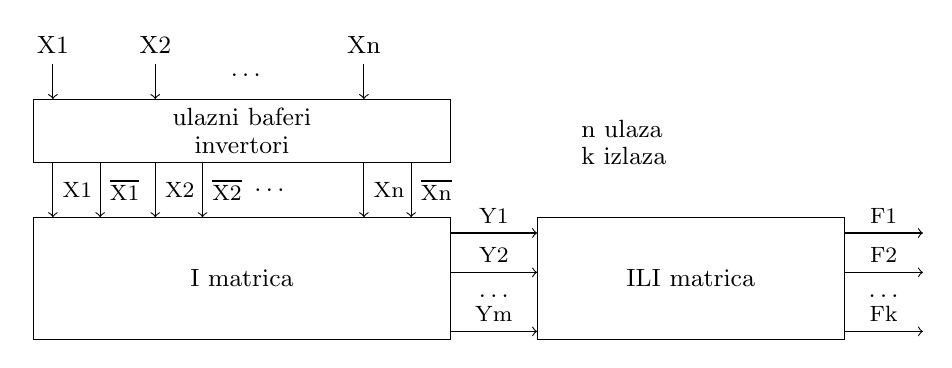
\begin{tikzpicture}[x=1cm,y=1cm,font=\fontsize{9}{10}\selectfont]
\draw (0,2.25) rectangle (5.3,3.05);\node[align=center] at (2.65,2.65) {ulazni baferi\\invertori};
\draw (0,0) rectangle (5.3,1.55);\node at (2.65,.775) {I matrica};
\draw (6.4,0) rectangle (10.3,1.55);\node at (8.35,.775) {ILI matrica};
\node[align=left] at (7.5,2.5) {n ulaza\\k izlaza};
\draw[->] (0.25,3.5) node[above] {X1}--(0.25,3.05);
\draw[->] (1.55,3.5) node[above] {X2}--(1.55,3.05);
\draw[->] (4.2,3.5) node[above] {Xn}--(4.2,3.05);
\node at (2.7,3.35) {$\ldots$};
\node at (3,1.9) {$\ldots$};
\draw[->] (0.25,2.25)--(0.25,1.55) node[midway,right=0pt,font=\fontsize{8}{9}\selectfont] {X1};
\draw[->] (0.85,2.25)--(0.85,1.55) node[midway,right=0pt,font=\fontsize{8}{9}\selectfont] {$\overline{\mathrm{X1}}$};
\draw[->] (1.55,2.25)--(1.55,1.55) node[midway,right=0pt,font=\fontsize{8}{9}\selectfont] {X2};
\draw[->] (2.15,2.25)--(2.15,1.55) node[midway,right=0pt,font=\fontsize{8}{9}\selectfont] {$\overline{\mathrm{X2}}$};
\draw[->] (4.2,2.25)--(4.2,1.55) node[midway,right=0pt,font=\fontsize{8}{9}\selectfont] {Xn};
\draw[->] (4.8,2.25)--(4.8,1.55) node[midway,right=0pt,font=\fontsize{8}{9}\selectfont] {$\overline{\mathrm{Xn}}$};
\draw[->] (5.3,1.35)--(6.4,1.35) node[midway,above=0pt,font=\fontsize{8}{9}\selectfont] {Y1};
\draw[->] (10.3,1.35)--(11.3,1.35) node[midway,above=0pt,font=\fontsize{8}{9}\selectfont] {F1};
\draw[->] (5.3,0.85)--(6.4,0.85) node[midway,above=0pt,font=\fontsize{8}{9}\selectfont] {Y2};
\draw[->] (10.3,0.85)--(11.3,0.85) node[midway,above=0pt,font=\fontsize{8}{9}\selectfont] {F2};
\draw[->] (5.3,0.1)--(6.4,0.1) node[midway,above=0pt,font=\fontsize{8}{9}\selectfont] {Ym};
\draw[->] (10.3,0.1)--(11.3,0.1) node[midway,above=0pt,font=\fontsize{8}{9}\selectfont] {Fk};
\node at (5.85,.55) {$\ldots$};\node at (10.8,.55) {$\ldots$};
\end{tikzpicture}
\par\vspace{2mm}
\raggedright Šta i koliko može da se programira zavisi od tipa komponente.\par\vspace{2mm}
Da li su obe matrice programabilne?\\
Da li je samo I odnosno ILI matrica programabilna?\\
Koliko su programabilne?\\
Šta može da učestvuje u Y i koliko ih ima (m?)? Koliko ulaza u I kola.\\
Šta može da učestvuje u F i koliko? Koliko ulaza u ILI kola.
\end{frame}

\slajdid{07-s006}
\begin{frame}[label=07-s006]
\centering\begin{tikzpicture}[x=1cm,y=1cm,font=\fontsize{11}{13}\selectfont]
\node[anchor=west] at (0,0) {PLA – \textcolor{DEplava}{P}rogrammable \textcolor{DEplava}{L}ogic \textcolor{DEplava}{A}rray};
\node[anchor=west] at (0,-0.65) {PAL – \textcolor{DEplava}{P}rogrammable \textcolor{DEplava}{A}rray \textcolor{DEplava}{L}ogic};
\node[anchor=west] at (0,-1.3) {GAL – \textcolor{DEplava}{G}eneric \textcolor{DEplava}{A}rray \textcolor{DEplava}{L}ogic};
\node[anchor=west] at (0,-2.05) {CPLD – \textcolor{DEplava}{C}omplex \textcolor{DEplava}{P}rogrammable \textcolor{DEplava}{L}ogic \textcolor{DEplava}{D}evice};
\node[anchor=west] at (0,-2.7) {FPGA– \textcolor{DEplava}{F}ild \textcolor{DEplava}{P}rogrammable \textcolor{DEplava}{G}ate \textcolor{DEplava}{A}rray};
\node[anchor=west] at (0,-3.75) {ROM – \textcolor{DEplava}{R}ead \textcolor{DEplava}{O}nly \textcolor{DEplava}{M}\textcolor{DEcrvena}{emory}};
\node[anchor=west] at (0,-4.4) {PROM – \textcolor{DEplava}{P}rogrammable \textcolor{DEplava}{ROM}};
\node[anchor=west] at (0,-5.2) {EEPROM – \textcolor{DEplava}{E}lectrically \textcolor{DEplava}{EPROM}};
\node[anchor=west] at (0,-6.15) {ASIC– \textcolor{DEplava}{A}pplication \textcolor{DEplava}{S}pecific Integrated \textcolor{DEplava}{C}ircuit};
\draw[DEplava,decorate,decoration={brace,amplitude=5pt}] (9.0,0.25)--(9.0,-1.6) node[midway,right=8pt,text=DEtekst] {PLD};
\draw[DEplava,decorate,decoration={brace,amplitude=5pt}] (11,-1.8)--(11,-3.0) node[midway,right=8pt,text=DEtekst] {CPLD};
\draw[DEplava,decorate,decoration={brace,amplitude=5pt}] (9,-3.45)--(9,-5.5) node[midway,right=8pt,text=DEtekst] {\textcolor{DEcrvena}{Memory}};
\draw[DEplava,decorate,decoration={brace,amplitude=5pt}] (10.5,-5.85)--(10.5,-6.45) node[midway,right=8pt,text=DEtekst] {ASIC};
\end{tikzpicture}

\end{frame}

\slajdid{07-s007}
\begin{frame}[label=07-s007]{Primer jedne PAL komponente}
\gusttekst\setlength{\parskip}{1pt}\begin{columns}[c,onlytextwidth]
\column{.61\textwidth}\centering\begin{tikzpicture}[remember picture,x=1cm,y=1cm,font=\fontsize{8}{9}\selectfont,line width=.25pt,>=Latex]
\draw ( 0.0,.10)--(0.0,-4.9);
\draw[DEplava!55] (0.0,.10)--(0.0,0.1);
\node[text=DEplava,inner sep=.2pt,fill=white] at (0.0,0.2) {0};
\draw ( 0.08,.10)--(0.08,-4.9);
\draw[DEplava!55] (0.08,.10)--(0.08,0.36);
\node[text=DEplava,inner sep=.2pt,fill=white] at (0.08,0.46) {1};
\draw ( 0.16,.10)--(0.16,-4.9);
\draw[DEplava!55] (0.16,.10)--(0.16,0.62);
\node[text=DEplava,inner sep=.2pt,fill=white] at (0.16,0.72) {2};
\draw ( 0.24,.10)--(0.24,-4.9);
\draw[DEplava!55] (0.24,.10)--(0.24,0.88);
\node[text=DEplava,inner sep=.2pt,fill=white] at (0.24,0.98) {3};
\draw ( 0.32,.10)--(0.32,-4.9);
\draw[DEplava!55] (0.32,.10)--(0.32,1.14);
\node[text=DEplava,inner sep=.2pt,fill=white] at (0.32,1.24) {4};
\draw ( 0.4,.10)--(0.4,-4.9);
\draw[DEplava!55] (0.4,.10)--(0.4,0.1);
\node[text=DEplava,inner sep=.2pt,fill=white] at (0.4,0.2) {5};
\draw ( 0.48,.10)--(0.48,-4.9);
\draw[DEplava!55] (0.48,.10)--(0.48,0.36);
\node[text=DEplava,inner sep=.2pt,fill=white] at (0.48,0.46) {6};
\draw ( 0.56,.10)--(0.56,-4.9);
\draw[DEplava!55] (0.56,.10)--(0.56,0.62);
\node[text=DEplava,inner sep=.2pt,fill=white] at (0.56,0.72) {7};
\draw ( 0.64,.10)--(0.64,-4.9);
\draw[DEplava!55] (0.64,.10)--(0.64,0.88);
\node[text=DEplava,inner sep=.2pt,fill=white] at (0.64,0.98) {8};
\draw ( 0.72,.10)--(0.72,-4.9);
\draw[DEplava!55] (0.72,.10)--(0.72,1.14);
\node[text=DEplava,inner sep=.2pt,fill=white] at (0.72,1.24) {9};
\draw ( 0.8,.10)--(0.8,-4.9);
\draw[DEplava!55] (0.8,.10)--(0.8,0.1);
\node[text=DEplava,inner sep=.2pt,fill=white] at (0.8,0.2) {10};
\draw ( 0.88,.10)--(0.88,-4.9);
\draw[DEplava!55] (0.88,.10)--(0.88,0.36);
\node[text=DEplava,inner sep=.2pt,fill=white] at (0.88,0.46) {11};
\draw ( 0.96,.10)--(0.96,-4.9);
\draw[DEplava!55] (0.96,.10)--(0.96,0.62);
\node[text=DEplava,inner sep=.2pt,fill=white] at (0.96,0.72) {12};
\draw ( 1.04,.10)--(1.04,-4.9);
\draw[DEplava!55] (1.04,.10)--(1.04,0.88);
\node[text=DEplava,inner sep=.2pt,fill=white] at (1.04,0.98) {13};
\draw ( 1.12,.10)--(1.12,-4.9);
\draw[DEplava!55] (1.12,.10)--(1.12,1.14);
\node[text=DEplava,inner sep=.2pt,fill=white] at (1.12,1.24) {14};
\draw ( 1.2,.10)--(1.2,-4.9);
\draw[DEplava!55] (1.2,.10)--(1.2,0.1);
\node[text=DEplava,inner sep=.2pt,fill=white] at (1.2,0.2) {15};
\draw ( 1.28,.10)--(1.28,-4.9);
\draw[DEplava!55] (1.28,.10)--(1.28,0.36);
\node[text=DEplava,inner sep=.2pt,fill=white] at (1.28,0.46) {16};
\draw ( 1.36,.10)--(1.36,-4.9);
\draw[DEplava!55] (1.36,.10)--(1.36,0.62);
\node[text=DEplava,inner sep=.2pt,fill=white] at (1.36,0.72) {17};
\draw ( 1.44,.10)--(1.44,-4.9);
\draw[DEplava!55] (1.44,.10)--(1.44,0.88);
\node[text=DEplava,inner sep=.2pt,fill=white] at (1.44,0.98) {18};
\draw ( 1.52,.10)--(1.52,-4.9);
\draw[DEplava!55] (1.52,.10)--(1.52,1.14);
\node[text=DEplava,inner sep=.2pt,fill=white] at (1.52,1.24) {19};
\draw ( 1.6,.10)--(1.6,-4.9);
\draw[DEplava!55] (1.6,.10)--(1.6,0.1);
\node[text=DEplava,inner sep=.2pt,fill=white] at (1.6,0.2) {20};
\draw ( 1.68,.10)--(1.68,-4.9);
\draw[DEplava!55] (1.68,.10)--(1.68,0.36);
\node[text=DEplava,inner sep=.2pt,fill=white] at (1.68,0.46) {21};
\draw ( 1.76,.10)--(1.76,-4.9);
\draw[DEplava!55] (1.76,.10)--(1.76,0.62);
\node[text=DEplava,inner sep=.2pt,fill=white] at (1.76,0.72) {22};
\draw ( 1.84,.10)--(1.84,-4.9);
\draw[DEplava!55] (1.84,.10)--(1.84,0.88);
\node[text=DEplava,inner sep=.2pt,fill=white] at (1.84,0.98) {23};
\draw ( 1.92,.10)--(1.92,-4.9);
\draw[DEplava!55] (1.92,.10)--(1.92,1.14);
\node[text=DEplava,inner sep=.2pt,fill=white] at (1.92,1.24) {24};
\draw ( 2.0,.10)--(2.0,-4.9);
\draw[DEplava!55] (2.0,.10)--(2.0,0.1);
\node[text=DEplava,inner sep=.2pt,fill=white] at (2.0,0.2) {25};
\draw ( 2.08,.10)--(2.08,-4.9);
\draw[DEplava!55] (2.08,.10)--(2.08,0.36);
\node[text=DEplava,inner sep=.2pt,fill=white] at (2.08,0.46) {26};
\draw ( 2.16,.10)--(2.16,-4.9);
\draw[DEplava!55] (2.16,.10)--(2.16,0.62);
\node[text=DEplava,inner sep=.2pt,fill=white] at (2.16,0.72) {27};
\draw ( 2.24,.10)--(2.24,-4.9);
\draw[DEplava!55] (2.24,.10)--(2.24,0.88);
\node[text=DEplava,inner sep=.2pt,fill=white] at (2.24,0.98) {28};
\draw ( 2.32,.10)--(2.32,-4.9);
\draw[DEplava!55] (2.32,.10)--(2.32,1.14);
\node[text=DEplava,inner sep=.2pt,fill=white] at (2.32,1.24) {29};
\draw ( 2.4,.10)--(2.4,-4.9);
\draw[DEplava!55] (2.4,.10)--(2.4,0.1);
\node[text=DEplava,inner sep=.2pt,fill=white] at (2.4,0.2) {30};
\draw ( 2.48,.10)--(2.48,-4.9);
\draw[DEplava!55] (2.48,.10)--(2.48,0.36);
\node[text=DEplava,inner sep=.2pt,fill=white] at (2.48,0.46) {31};
\draw[DEplava!55] (-0.23,-0.0)--(-.10,-0.0);
\node[fill=white,inner sep=.2pt,text=DEplava] at (-0.23,-0.0) {0};
\draw (-.10,-0.0)--(2.55,-0.0);
\draw[fill=white] (2.55,-0.024)--(2.63,-0.024) arc(-90:90:.024)--(2.55,0.024)--cycle;
\draw (2.654,-0.0)--(3.47,-0.0)--(3.47,-0.15);
\draw[DEplava!55] (-0.61,-0.06)--(-.10,-0.06);
\node[fill=white,inner sep=.2pt,text=DEplava] at (-0.61,-0.06) {1};
\draw (-.10,-0.06)--(2.55,-0.06);
\draw[fill=white] (2.55,-0.08399999999999999)--(2.63,-0.08399999999999999) arc(-90:90:.024)--(2.55,-0.036)--cycle;
\draw (2.654,-0.06)--(2.73,-0.06)--(2.73,-0.12)--(2.87,-0.12);
\draw[DEplava!55] (-0.99,-0.12)--(-.10,-0.12);
\node[fill=white,inner sep=.2pt,text=DEplava] at (-0.99,-0.12) {2};
\draw (-.10,-0.12)--(2.55,-0.12);
\draw[fill=white] (2.55,-0.144)--(2.63,-0.144) arc(-90:90:.024)--(2.55,-0.096)--cycle;
\draw (2.654,-0.12)--(2.73,-0.12)--(2.73,-0.16)--(2.87,-0.16);
\draw[DEplava!55] (-1.37,-0.18)--(-.10,-0.18);
\node[fill=white,inner sep=.2pt,text=DEplava] at (-1.37,-0.18) {3};
\draw (-.10,-0.18)--(2.55,-0.18);
\draw[fill=white] (2.55,-0.204)--(2.63,-0.204) arc(-90:90:.024)--(2.55,-0.156)--cycle;
\draw (2.654,-0.18)--(2.73,-0.18)--(2.73,-0.2)--(2.87,-0.2);
\draw[DEplava!55] (-1.75,-0.24)--(-.10,-0.24);
\node[fill=white,inner sep=.2pt,text=DEplava] at (-1.75,-0.24) {4};
\draw (-.10,-0.24)--(2.55,-0.24);
\draw[fill=white] (2.55,-0.264)--(2.63,-0.264) arc(-90:90:.024)--(2.55,-0.216)--cycle;
\draw (2.654,-0.24)--(2.73,-0.24)--(2.73,-0.24)--(2.87,-0.24);
\draw[DEplava!55] (-0.23,-0.3)--(-.10,-0.3);
\node[fill=white,inner sep=.2pt,text=DEplava] at (-0.23,-0.3) {5};
\draw (-.10,-0.3)--(2.55,-0.3);
\draw[fill=white] (2.55,-0.324)--(2.63,-0.324) arc(-90:90:.024)--(2.55,-0.27599999999999997)--cycle;
\draw (2.654,-0.3)--(2.73,-0.3)--(2.73,-0.28)--(2.87,-0.28);
\draw[DEplava!55] (-0.61,-0.36)--(-.10,-0.36);
\node[fill=white,inner sep=.2pt,text=DEplava] at (-0.61,-0.36) {6};
\draw (-.10,-0.36)--(2.55,-0.36);
\draw[fill=white] (2.55,-0.384)--(2.63,-0.384) arc(-90:90:.024)--(2.55,-0.33599999999999997)--cycle;
\draw (2.654,-0.36)--(2.73,-0.36)--(2.73,-0.32)--(2.87,-0.32);
\draw[DEplava!55] (-0.99,-0.42)--(-.10,-0.42);
\node[fill=white,inner sep=.2pt,text=DEplava] at (-0.99,-0.42) {7};
\draw (-.10,-0.42)--(2.55,-0.42);
\draw[fill=white] (2.55,-0.444)--(2.63,-0.444) arc(-90:90:.024)--(2.55,-0.39599999999999996)--cycle;
\draw (2.654,-0.42)--(2.73,-0.42)--(2.73,-0.36)--(2.87,-0.36);
\draw[fill=white] (2.82,-0.42) .. controls (3.02,-0.42) and (3.16,-0.39) .. (3.28,-0.24) .. controls (3.16,-0.09) and (3.02,-0.06) .. (2.82,-0.06) .. controls (2.94,-0.19999999999999998) and (2.94,-0.27999999999999997) .. cycle;
\draw (3.28,-0.24)--(3.38,-0.24);
\draw[fill=white] (3.38,-0.32999999999999996)--(3.61,-0.24)--(3.38,-0.15)--cycle;\draw[fill=white] (3.64,-0.24) circle(.03);
\draw (3.67,-0.24)--(4.10,-0.24);
\node[anchor=west,inner sep=1pt] at (4.1,-0.24) {O1};
\node[anchor=south,text=DEplava,inner sep=0pt] at (3.95,-0.22) {(19)};
\draw (-2.25,-0.51)--(-2.02,-0.51);
\draw[fill=white] (-2.02,-0.6)--(-1.80,-0.51)--(-2.02,-0.42000000000000004)--cycle;
\draw[fill=white] (-1.80,-0.5650000000000001) circle(.025);
\draw (-1.84,-0.455)--(0.0,-0.455);
\draw (-1.775,-0.5650000000000001)--(0.08,-0.5650000000000001);
\fill (0.0,-0.455) circle(.012);\fill (0.08,-0.5650000000000001) circle(.012);
\node[anchor=east,inner sep=1pt] at (-2.25,-0.51) {I2};
\node[anchor=south,text=DEplava,inner sep=0pt] at (-2.30,-0.45) {(2)};
\draw[fill=white] (3.63,-0.6)--(3.40,-0.51)--(3.63,-0.42000000000000004)--cycle;
\draw[fill=white] (3.40,-0.5650000000000001) circle(.025);
\draw (3.44,-0.455)--(0.16,-0.455);
\draw (3.375,-0.5650000000000001)--(0.24,-0.5650000000000001);
\fill (0.16,-0.455) circle(.012);\fill (0.24,-0.5650000000000001) circle(.012);
\draw (-2.25,1.55)--(4.35,1.55)--(4.35,-0.51)--(3.63,-0.51);\node[anchor=east] at (-2.25,1.55) {I1};\node[anchor=south,text=DEplava] at (-2.3,1.57) {(1)};
\draw[DEplava!55] (-1.37,-0.6)--(-.10,-0.6);
\node[fill=white,inner sep=.2pt,text=DEplava] at (-1.37,-0.6) {8};
\draw (-.10,-0.6)--(2.55,-0.6);
\draw[fill=white] (2.55,-0.624)--(2.63,-0.624) arc(-90:90:.024)--(2.55,-0.576)--cycle;
\draw (2.654,-0.6)--(3.47,-0.6)--(3.47,-0.75);
\draw[DEplava!55] (-1.75,-0.6599999999999999)--(-.10,-0.6599999999999999);
\node[fill=white,inner sep=.2pt,text=DEplava] at (-1.75,-0.6599999999999999) {9};
\draw (-.10,-0.6599999999999999)--(2.55,-0.6599999999999999);
\draw[fill=white] (2.55,-0.6839999999999999)--(2.63,-0.6839999999999999) arc(-90:90:.024)--(2.55,-0.6359999999999999)--cycle;
\draw (2.654,-0.6599999999999999)--(2.73,-0.6599999999999999)--(2.73,-0.72)--(2.87,-0.72);
\draw[DEplava!55] (-0.23,-0.72)--(-.10,-0.72);
\node[fill=white,inner sep=.2pt,text=DEplava] at (-0.23,-0.72) {10};
\draw (-.10,-0.72)--(2.55,-0.72);
\draw[fill=white] (2.55,-0.744)--(2.63,-0.744) arc(-90:90:.024)--(2.55,-0.696)--cycle;
\draw (2.654,-0.72)--(2.73,-0.72)--(2.73,-0.76)--(2.87,-0.76);
\draw[DEplava!55] (-0.61,-0.78)--(-.10,-0.78);
\node[fill=white,inner sep=.2pt,text=DEplava] at (-0.61,-0.78) {11};
\draw (-.10,-0.78)--(2.55,-0.78);
\draw[fill=white] (2.55,-0.804)--(2.63,-0.804) arc(-90:90:.024)--(2.55,-0.756)--cycle;
\draw (2.654,-0.78)--(2.73,-0.78)--(2.73,-0.7999999999999999)--(2.87,-0.7999999999999999);
\draw[DEplava!55] (-0.99,-0.84)--(-.10,-0.84);
\node[fill=white,inner sep=.2pt,text=DEplava] at (-0.99,-0.84) {12};
\draw (-.10,-0.84)--(2.55,-0.84);
\draw[fill=white] (2.55,-0.864)--(2.63,-0.864) arc(-90:90:.024)--(2.55,-0.816)--cycle;
\draw (2.654,-0.84)--(2.73,-0.84)--(2.73,-0.84)--(2.87,-0.84);
\draw[DEplava!55] (-1.37,-0.8999999999999999)--(-.10,-0.8999999999999999);
\node[fill=white,inner sep=.2pt,text=DEplava] at (-1.37,-0.8999999999999999) {13};
\draw (-.10,-0.8999999999999999)--(2.55,-0.8999999999999999);
\draw[fill=white] (2.55,-0.9239999999999999)--(2.63,-0.9239999999999999) arc(-90:90:.024)--(2.55,-0.8759999999999999)--cycle;
\draw (2.654,-0.8999999999999999)--(2.73,-0.8999999999999999)--(2.73,-0.88)--(2.87,-0.88);
\draw[DEplava!55] (-1.75,-0.96)--(-.10,-0.96);
\node[fill=white,inner sep=.2pt,text=DEplava] at (-1.75,-0.96) {14};
\draw (-.10,-0.96)--(2.55,-0.96);
\draw[fill=white] (2.55,-0.984)--(2.63,-0.984) arc(-90:90:.024)--(2.55,-0.9359999999999999)--cycle;
\draw (2.654,-0.96)--(2.73,-0.96)--(2.73,-0.9199999999999999)--(2.87,-0.9199999999999999);
\draw[DEplava!55] (-0.23,-1.02)--(-.10,-1.02);
\node[fill=white,inner sep=.2pt,text=DEplava] at (-0.23,-1.02) {15};
\draw (-.10,-1.02)--(2.55,-1.02);
\draw[fill=white] (2.55,-1.044)--(2.63,-1.044) arc(-90:90:.024)--(2.55,-0.996)--cycle;
\draw (2.654,-1.02)--(2.73,-1.02)--(2.73,-0.96)--(2.87,-0.96);
\draw[fill=white] (2.82,-1.02) .. controls (3.02,-1.02) and (3.16,-0.99) .. (3.28,-0.84) .. controls (3.16,-0.69) and (3.02,-0.6599999999999999) .. (2.82,-0.6599999999999999) .. controls (2.94,-0.7999999999999999) and (2.94,-0.88) .. cycle;
\draw (3.28,-0.84)--(3.38,-0.84);
\draw[fill=white] (3.38,-0.9299999999999999)--(3.61,-0.84)--(3.38,-0.75)--cycle;\draw[fill=white] (3.64,-0.84) circle(.03);
\draw (3.67,-0.84)--(4.10,-0.84);
\node[anchor=west,inner sep=1pt] at (4.1,-0.84) {IO2};
\node[anchor=south,text=DEplava,inner sep=0pt] at (3.95,-0.82) {(18)};
\draw (-2.25,-1.1099999999999999)--(-2.02,-1.1099999999999999);
\draw[fill=white] (-2.02,-1.2)--(-1.80,-1.1099999999999999)--(-2.02,-1.0199999999999998)--cycle;
\draw[fill=white] (-1.80,-1.1649999999999998) circle(.025);
\draw (-1.84,-1.055)--(0.32,-1.055);
\draw (-1.775,-1.1649999999999998)--(0.4,-1.1649999999999998);
\fill (0.32,-1.055) circle(.012);\fill (0.4,-1.1649999999999998) circle(.012);
\node[anchor=east,inner sep=1pt] at (-2.25,-1.1099999999999999) {I3};
\node[anchor=south,text=DEplava,inner sep=0pt] at (-2.30,-1.0499999999999998) {(3)};
\draw[fill=white] (3.63,-1.2)--(3.40,-1.1099999999999999)--(3.63,-1.0199999999999998)--cycle;
\draw[fill=white] (3.40,-1.1649999999999998) circle(.025);
\draw (3.44,-1.055)--(0.48,-1.055);
\draw (3.375,-1.1649999999999998)--(0.56,-1.1649999999999998);
\fill (0.48,-1.055) circle(.012);\fill (0.56,-1.1649999999999998) circle(.012);
\draw (3.85,-0.84)--(3.85,-1.1099999999999999)--(3.63,-1.1099999999999999);\fill (3.85,-0.84) circle(.012);
\draw[DEplava!55] (-0.61,-1.2)--(-.10,-1.2);
\node[fill=white,inner sep=.2pt,text=DEplava] at (-0.61,-1.2) {16};
\draw (-.10,-1.2)--(2.55,-1.2);
\draw[fill=white] (2.55,-1.224)--(2.63,-1.224) arc(-90:90:.024)--(2.55,-1.176)--cycle;
\draw (2.654,-1.2)--(3.47,-1.2)--(3.47,-1.3499999999999999);
\draw[DEplava!55] (-0.99,-1.26)--(-.10,-1.26);
\node[fill=white,inner sep=.2pt,text=DEplava] at (-0.99,-1.26) {17};
\draw (-.10,-1.26)--(2.55,-1.26);
\draw[fill=white] (2.55,-1.284)--(2.63,-1.284) arc(-90:90:.024)--(2.55,-1.236)--cycle;
\draw (2.654,-1.26)--(2.73,-1.26)--(2.73,-1.3199999999999998)--(2.87,-1.3199999999999998);
\draw[DEplava!55] (-1.37,-1.3199999999999998)--(-.10,-1.3199999999999998);
\node[fill=white,inner sep=.2pt,text=DEplava] at (-1.37,-1.3199999999999998) {18};
\draw (-.10,-1.3199999999999998)--(2.55,-1.3199999999999998);
\draw[fill=white] (2.55,-1.3439999999999999)--(2.63,-1.3439999999999999) arc(-90:90:.024)--(2.55,-1.2959999999999998)--cycle;
\draw (2.654,-1.3199999999999998)--(2.73,-1.3199999999999998)--(2.73,-1.3599999999999999)--(2.87,-1.3599999999999999);
\draw[DEplava!55] (-1.75,-1.38)--(-.10,-1.38);
\node[fill=white,inner sep=.2pt,text=DEplava] at (-1.75,-1.38) {19};
\draw (-.10,-1.38)--(2.55,-1.38);
\draw[fill=white] (2.55,-1.404)--(2.63,-1.404) arc(-90:90:.024)--(2.55,-1.3559999999999999)--cycle;
\draw (2.654,-1.38)--(2.73,-1.38)--(2.73,-1.4)--(2.87,-1.4);
\draw[DEplava!55] (-0.23,-1.44)--(-.10,-1.44);
\node[fill=white,inner sep=.2pt,text=DEplava] at (-0.23,-1.44) {20};
\draw (-.10,-1.44)--(2.55,-1.44);
\draw[fill=white] (2.55,-1.464)--(2.63,-1.464) arc(-90:90:.024)--(2.55,-1.416)--cycle;
\draw (2.654,-1.44)--(2.73,-1.44)--(2.73,-1.44)--(2.87,-1.44);
\draw[DEplava!55] (-0.61,-1.5)--(-.10,-1.5);
\node[fill=white,inner sep=.2pt,text=DEplava] at (-0.61,-1.5) {21};
\draw (-.10,-1.5)--(2.55,-1.5);
\draw[fill=white] (2.55,-1.524)--(2.63,-1.524) arc(-90:90:.024)--(2.55,-1.476)--cycle;
\draw (2.654,-1.5)--(2.73,-1.5)--(2.73,-1.4799999999999998)--(2.87,-1.4799999999999998);
\draw[DEplava!55] (-0.99,-1.56)--(-.10,-1.56);
\node[fill=white,inner sep=.2pt,text=DEplava] at (-0.99,-1.56) {22};
\draw (-.10,-1.56)--(2.55,-1.56);
\draw[fill=white] (2.55,-1.584)--(2.63,-1.584) arc(-90:90:.024)--(2.55,-1.536)--cycle;
\draw (2.654,-1.56)--(2.73,-1.56)--(2.73,-1.5199999999999998)--(2.87,-1.5199999999999998);
\draw[DEplava!55] (-1.37,-1.6199999999999999)--(-.10,-1.6199999999999999);
\node[fill=white,inner sep=.2pt,text=DEplava] at (-1.37,-1.6199999999999999) {23};
\draw (-.10,-1.6199999999999999)--(2.55,-1.6199999999999999);
\draw[fill=white] (2.55,-1.644)--(2.63,-1.644) arc(-90:90:.024)--(2.55,-1.5959999999999999)--cycle;
\draw (2.654,-1.6199999999999999)--(2.73,-1.6199999999999999)--(2.73,-1.5599999999999998)--(2.87,-1.5599999999999998);
\draw[fill=white] (2.82,-1.6199999999999999) .. controls (3.02,-1.6199999999999999) and (3.16,-1.5899999999999999) .. (3.28,-1.44) .. controls (3.16,-1.29) and (3.02,-1.26) .. (2.82,-1.26) .. controls (2.94,-1.4) and (2.94,-1.48) .. cycle;
\draw (3.28,-1.44)--(3.38,-1.44);
\draw[fill=white] (3.38,-1.53)--(3.61,-1.44)--(3.38,-1.3499999999999999)--cycle;\draw[fill=white] (3.64,-1.44) circle(.03);
\draw (3.67,-1.44)--(4.10,-1.44);
\node[anchor=west,inner sep=1pt] at (4.1,-1.44) {IO3};
\node[anchor=south,text=DEplava,inner sep=0pt] at (3.95,-1.42) {(17)};
\draw (-2.25,-1.71)--(-2.02,-1.71);
\draw[fill=white] (-2.02,-1.8)--(-1.80,-1.71)--(-2.02,-1.6199999999999999)--cycle;
\draw[fill=white] (-1.80,-1.765) circle(.025);
\draw (-1.84,-1.655)--(0.64,-1.655);
\draw (-1.775,-1.765)--(0.72,-1.765);
\fill (0.64,-1.655) circle(.012);\fill (0.72,-1.765) circle(.012);
\node[anchor=east,inner sep=1pt] at (-2.25,-1.71) {I4};
\node[anchor=south,text=DEplava,inner sep=0pt] at (-2.30,-1.65) {(4)};
\draw[fill=white] (3.63,-1.8)--(3.40,-1.71)--(3.63,-1.6199999999999999)--cycle;
\draw[fill=white] (3.40,-1.765) circle(.025);
\draw (3.44,-1.655)--(0.8,-1.655);
\draw (3.375,-1.765)--(0.88,-1.765);
\fill (0.8,-1.655) circle(.012);\fill (0.88,-1.765) circle(.012);
\draw (3.85,-1.44)--(3.85,-1.71)--(3.63,-1.71);\fill (3.85,-1.44) circle(.012);
\draw[DEplava!55] (-1.75,-1.7999999999999998)--(-.10,-1.7999999999999998);
\node[fill=white,inner sep=.2pt,text=DEplava] at (-1.75,-1.7999999999999998) {24};
\draw (-.10,-1.7999999999999998)--(2.55,-1.7999999999999998);
\draw[fill=white] (2.55,-1.8239999999999998)--(2.63,-1.8239999999999998) arc(-90:90:.024)--(2.55,-1.7759999999999998)--cycle;
\draw (2.654,-1.7999999999999998)--(3.47,-1.7999999999999998)--(3.47,-1.95);
\draw[DEplava!55] (-0.23,-1.8599999999999999)--(-.10,-1.8599999999999999);
\node[fill=white,inner sep=.2pt,text=DEplava] at (-0.23,-1.8599999999999999) {25};
\draw (-.10,-1.8599999999999999)--(2.55,-1.8599999999999999);
\draw[fill=white] (2.55,-1.884)--(2.63,-1.884) arc(-90:90:.024)--(2.55,-1.8359999999999999)--cycle;
\draw (2.654,-1.8599999999999999)--(2.73,-1.8599999999999999)--(2.73,-1.92)--(2.87,-1.92);
\draw[DEplava!55] (-0.61,-1.92)--(-.10,-1.92);
\node[fill=white,inner sep=.2pt,text=DEplava] at (-0.61,-1.92) {26};
\draw (-.10,-1.92)--(2.55,-1.92);
\draw[fill=white] (2.55,-1.944)--(2.63,-1.944) arc(-90:90:.024)--(2.55,-1.896)--cycle;
\draw (2.654,-1.92)--(2.73,-1.92)--(2.73,-1.96)--(2.87,-1.96);
\draw[DEplava!55] (-0.99,-1.9799999999999998)--(-.10,-1.9799999999999998);
\node[fill=white,inner sep=.2pt,text=DEplava] at (-0.99,-1.9799999999999998) {27};
\draw (-.10,-1.9799999999999998)--(2.55,-1.9799999999999998);
\draw[fill=white] (2.55,-2.0039999999999996)--(2.63,-2.0039999999999996) arc(-90:90:.024)--(2.55,-1.9559999999999997)--cycle;
\draw (2.654,-1.9799999999999998)--(2.73,-1.9799999999999998)--(2.73,-2.0)--(2.87,-2.0);
\draw[DEplava!55] (-1.37,-2.04)--(-.10,-2.04);
\node[fill=white,inner sep=.2pt,text=DEplava] at (-1.37,-2.04) {28};
\draw (-.10,-2.04)--(2.55,-2.04);
\draw[fill=white] (2.55,-2.064)--(2.63,-2.064) arc(-90:90:.024)--(2.55,-2.016)--cycle;
\draw (2.654,-2.04)--(2.73,-2.04)--(2.73,-2.04)--(2.87,-2.04);
\draw[DEplava!55] (-1.75,-2.0999999999999996)--(-.10,-2.0999999999999996);
\node[fill=white,inner sep=.2pt,text=DEplava] at (-1.75,-2.0999999999999996) {29};
\draw (-.10,-2.0999999999999996)--(2.55,-2.0999999999999996);
\draw[fill=white] (2.55,-2.1239999999999997)--(2.63,-2.1239999999999997) arc(-90:90:.024)--(2.55,-2.0759999999999996)--cycle;
\draw (2.654,-2.0999999999999996)--(2.73,-2.0999999999999996)--(2.73,-2.08)--(2.87,-2.08);
\draw[DEplava!55] (-0.23,-2.1599999999999997)--(-.10,-2.1599999999999997);
\node[fill=white,inner sep=.2pt,text=DEplava] at (-0.23,-2.1599999999999997) {30};
\draw (-.10,-2.1599999999999997)--(2.55,-2.1599999999999997);
\draw[fill=white] (2.55,-2.1839999999999997)--(2.63,-2.1839999999999997) arc(-90:90:.024)--(2.55,-2.1359999999999997)--cycle;
\draw (2.654,-2.1599999999999997)--(2.73,-2.1599999999999997)--(2.73,-2.12)--(2.87,-2.12);
\draw[DEplava!55] (-0.61,-2.2199999999999998)--(-.10,-2.2199999999999998);
\node[fill=white,inner sep=.2pt,text=DEplava] at (-0.61,-2.2199999999999998) {31};
\draw (-.10,-2.2199999999999998)--(2.55,-2.2199999999999998);
\draw[fill=white] (2.55,-2.2439999999999998)--(2.63,-2.2439999999999998) arc(-90:90:.024)--(2.55,-2.1959999999999997)--cycle;
\draw (2.654,-2.2199999999999998)--(2.73,-2.2199999999999998)--(2.73,-2.16)--(2.87,-2.16);
\draw[fill=white] (2.82,-2.22) .. controls (3.02,-2.22) and (3.16,-2.19) .. (3.28,-2.04) .. controls (3.16,-1.8900000000000001) and (3.02,-1.86) .. (2.82,-1.86) .. controls (2.94,-2.0) and (2.94,-2.08) .. cycle;
\draw (3.28,-2.04)--(3.38,-2.04);
\draw[fill=white] (3.38,-2.13)--(3.61,-2.04)--(3.38,-1.95)--cycle;\draw[fill=white] (3.64,-2.04) circle(.03);
\draw (3.67,-2.04)--(4.10,-2.04);
\node[anchor=west,inner sep=1pt] at (4.1,-2.04) {IO4};
\node[anchor=south,text=DEplava,inner sep=0pt] at (3.95,-2.02) {(16)};
\draw (-2.25,-2.3099999999999996)--(-2.02,-2.3099999999999996);
\draw[fill=white] (-2.02,-2.3999999999999995)--(-1.80,-2.3099999999999996)--(-2.02,-2.2199999999999998)--cycle;
\draw[fill=white] (-1.80,-2.3649999999999998) circle(.025);
\draw (-1.84,-2.2549999999999994)--(0.96,-2.2549999999999994);
\draw (-1.775,-2.3649999999999998)--(1.04,-2.3649999999999998);
\fill (0.96,-2.2549999999999994) circle(.012);\fill (1.04,-2.3649999999999998) circle(.012);
\node[anchor=east,inner sep=1pt] at (-2.25,-2.3099999999999996) {I5};
\node[anchor=south,text=DEplava,inner sep=0pt] at (-2.30,-2.2499999999999996) {(5)};
\draw[fill=white] (3.63,-2.3999999999999995)--(3.40,-2.3099999999999996)--(3.63,-2.2199999999999998)--cycle;
\draw[fill=white] (3.40,-2.3649999999999998) circle(.025);
\draw (3.44,-2.2549999999999994)--(1.12,-2.2549999999999994);
\draw (3.375,-2.3649999999999998)--(1.2,-2.3649999999999998);
\fill (1.12,-2.2549999999999994) circle(.012);\fill (1.2,-2.3649999999999998) circle(.012);
\draw (3.85,-2.04)--(3.85,-2.3099999999999996)--(3.63,-2.3099999999999996);\fill (3.85,-2.04) circle(.012);
\draw[DEplava!55] (-0.99,-2.4)--(-.10,-2.4);
\node[fill=white,inner sep=.2pt,text=DEplava] at (-0.99,-2.4) {32};
\draw (-.10,-2.4)--(2.55,-2.4);
\draw[fill=white] (2.55,-2.424)--(2.63,-2.424) arc(-90:90:.024)--(2.55,-2.376)--cycle;
\draw (2.654,-2.4)--(3.47,-2.4)--(3.47,-2.55);
\draw[DEplava!55] (-1.37,-2.46)--(-.10,-2.46);
\node[fill=white,inner sep=.2pt,text=DEplava] at (-1.37,-2.46) {33};
\draw (-.10,-2.46)--(2.55,-2.46);
\draw[fill=white] (2.55,-2.484)--(2.63,-2.484) arc(-90:90:.024)--(2.55,-2.436)--cycle;
\draw (2.654,-2.46)--(2.73,-2.46)--(2.73,-2.5199999999999996)--(2.87,-2.5199999999999996);
\draw[DEplava!55] (-1.75,-2.52)--(-.10,-2.52);
\node[fill=white,inner sep=.2pt,text=DEplava] at (-1.75,-2.52) {34};
\draw (-.10,-2.52)--(2.55,-2.52);
\draw[fill=white] (2.55,-2.544)--(2.63,-2.544) arc(-90:90:.024)--(2.55,-2.496)--cycle;
\draw (2.654,-2.52)--(2.73,-2.52)--(2.73,-2.5599999999999996)--(2.87,-2.5599999999999996);
\draw[DEplava!55] (-0.23,-2.58)--(-.10,-2.58);
\node[fill=white,inner sep=.2pt,text=DEplava] at (-0.23,-2.58) {35};
\draw (-.10,-2.58)--(2.55,-2.58);
\draw[fill=white] (2.55,-2.604)--(2.63,-2.604) arc(-90:90:.024)--(2.55,-2.556)--cycle;
\draw (2.654,-2.58)--(2.73,-2.58)--(2.73,-2.5999999999999996)--(2.87,-2.5999999999999996);
\draw[DEplava!55] (-0.61,-2.6399999999999997)--(-.10,-2.6399999999999997);
\node[fill=white,inner sep=.2pt,text=DEplava] at (-0.61,-2.6399999999999997) {36};
\draw (-.10,-2.6399999999999997)--(2.55,-2.6399999999999997);
\draw[fill=white] (2.55,-2.6639999999999997)--(2.63,-2.6639999999999997) arc(-90:90:.024)--(2.55,-2.6159999999999997)--cycle;
\draw (2.654,-2.6399999999999997)--(2.73,-2.6399999999999997)--(2.73,-2.6399999999999997)--(2.87,-2.6399999999999997);
\draw[DEplava!55] (-0.99,-2.6999999999999997)--(-.10,-2.6999999999999997);
\node[fill=white,inner sep=.2pt,text=DEplava] at (-0.99,-2.6999999999999997) {37};
\draw (-.10,-2.6999999999999997)--(2.55,-2.6999999999999997);
\draw[fill=white] (2.55,-2.7239999999999998)--(2.63,-2.7239999999999998) arc(-90:90:.024)--(2.55,-2.6759999999999997)--cycle;
\draw (2.654,-2.6999999999999997)--(2.73,-2.6999999999999997)--(2.73,-2.6799999999999997)--(2.87,-2.6799999999999997);
\draw[DEplava!55] (-1.37,-2.76)--(-.10,-2.76);
\node[fill=white,inner sep=.2pt,text=DEplava] at (-1.37,-2.76) {38};
\draw (-.10,-2.76)--(2.55,-2.76);
\draw[fill=white] (2.55,-2.784)--(2.63,-2.784) arc(-90:90:.024)--(2.55,-2.7359999999999998)--cycle;
\draw (2.654,-2.76)--(2.73,-2.76)--(2.73,-2.7199999999999998)--(2.87,-2.7199999999999998);
\draw[DEplava!55] (-1.75,-2.82)--(-.10,-2.82);
\node[fill=white,inner sep=.2pt,text=DEplava] at (-1.75,-2.82) {39};
\draw (-.10,-2.82)--(2.55,-2.82);
\draw[fill=white] (2.55,-2.844)--(2.63,-2.844) arc(-90:90:.024)--(2.55,-2.796)--cycle;
\draw (2.654,-2.82)--(2.73,-2.82)--(2.73,-2.76)--(2.87,-2.76);
\draw[fill=white] (2.82,-2.82) .. controls (3.02,-2.82) and (3.16,-2.7899999999999996) .. (3.28,-2.6399999999999997) .. controls (3.16,-2.4899999999999998) and (3.02,-2.4599999999999995) .. (2.82,-2.4599999999999995) .. controls (2.94,-2.5999999999999996) and (2.94,-2.6799999999999997) .. cycle;
\draw (3.28,-2.6399999999999997)--(3.38,-2.6399999999999997);
\draw[fill=white] (3.38,-2.7299999999999995)--(3.61,-2.6399999999999997)--(3.38,-2.55)--cycle;\draw[fill=white] (3.64,-2.6399999999999997) circle(.03);
\draw (3.67,-2.6399999999999997)--(4.10,-2.6399999999999997);
\node[anchor=west,inner sep=1pt] at (4.1,-2.6399999999999997) {IO5};
\node[anchor=south,text=DEplava,inner sep=0pt] at (3.95,-2.6199999999999997) {(15)};
\draw (-2.25,-2.91)--(-2.02,-2.91);
\draw[fill=white] (-2.02,-3.0)--(-1.80,-2.91)--(-2.02,-2.8200000000000003)--cycle;
\draw[fill=white] (-1.80,-2.9650000000000003) circle(.025);
\draw (-1.84,-2.855)--(1.28,-2.855);
\draw (-1.775,-2.9650000000000003)--(1.36,-2.9650000000000003);
\fill (1.28,-2.855) circle(.012);\fill (1.36,-2.9650000000000003) circle(.012);
\node[anchor=east,inner sep=1pt] at (-2.25,-2.91) {I6};
\node[anchor=south,text=DEplava,inner sep=0pt] at (-2.30,-2.85) {(6)};
\draw[fill=white] (3.63,-3.0)--(3.40,-2.91)--(3.63,-2.8200000000000003)--cycle;
\draw[fill=white] (3.40,-2.9650000000000003) circle(.025);
\draw (3.44,-2.855)--(1.44,-2.855);
\draw (3.375,-2.9650000000000003)--(1.52,-2.9650000000000003);
\fill (1.44,-2.855) circle(.012);\fill (1.52,-2.9650000000000003) circle(.012);
\draw (3.85,-2.6399999999999997)--(3.85,-2.91)--(3.63,-2.91);\fill (3.85,-2.6399999999999997) circle(.012);
\draw[DEplava!55] (-0.23,-3.0)--(-.10,-3.0);
\node[fill=white,inner sep=.2pt,text=DEplava] at (-0.23,-3.0) {40};
\draw (-.10,-3.0)--(2.55,-3.0);
\draw[fill=white] (2.55,-3.024)--(2.63,-3.024) arc(-90:90:.024)--(2.55,-2.976)--cycle;
\draw (2.654,-3.0)--(3.47,-3.0)--(3.47,-3.1500000000000004);
\draw[DEplava!55] (-0.61,-3.06)--(-.10,-3.06);
\node[fill=white,inner sep=.2pt,text=DEplava] at (-0.61,-3.06) {41};
\draw (-.10,-3.06)--(2.55,-3.06);
\draw[fill=white] (2.55,-3.084)--(2.63,-3.084) arc(-90:90:.024)--(2.55,-3.036)--cycle;
\draw (2.654,-3.06)--(2.73,-3.06)--(2.73,-3.12)--(2.87,-3.12);
\draw[DEplava!55] (-0.99,-3.12)--(-.10,-3.12);
\node[fill=white,inner sep=.2pt,text=DEplava] at (-0.99,-3.12) {42};
\draw (-.10,-3.12)--(2.55,-3.12);
\draw[fill=white] (2.55,-3.144)--(2.63,-3.144) arc(-90:90:.024)--(2.55,-3.096)--cycle;
\draw (2.654,-3.12)--(2.73,-3.12)--(2.73,-3.16)--(2.87,-3.16);
\draw[DEplava!55] (-1.37,-3.18)--(-.10,-3.18);
\node[fill=white,inner sep=.2pt,text=DEplava] at (-1.37,-3.18) {43};
\draw (-.10,-3.18)--(2.55,-3.18);
\draw[fill=white] (2.55,-3.204)--(2.63,-3.204) arc(-90:90:.024)--(2.55,-3.156)--cycle;
\draw (2.654,-3.18)--(2.73,-3.18)--(2.73,-3.2)--(2.87,-3.2);
\draw[DEplava!55] (-1.75,-3.24)--(-.10,-3.24);
\node[fill=white,inner sep=.2pt,text=DEplava] at (-1.75,-3.24) {44};
\draw (-.10,-3.24)--(2.55,-3.24);
\draw[fill=white] (2.55,-3.2640000000000002)--(2.63,-3.2640000000000002) arc(-90:90:.024)--(2.55,-3.216)--cycle;
\draw (2.654,-3.24)--(2.73,-3.24)--(2.73,-3.24)--(2.87,-3.24);
\draw[DEplava!55] (-0.23,-3.3)--(-.10,-3.3);
\node[fill=white,inner sep=.2pt,text=DEplava] at (-0.23,-3.3) {45};
\draw (-.10,-3.3)--(2.55,-3.3);
\draw[fill=white] (2.55,-3.324)--(2.63,-3.324) arc(-90:90:.024)--(2.55,-3.276)--cycle;
\draw (2.654,-3.3)--(2.73,-3.3)--(2.73,-3.2800000000000002)--(2.87,-3.2800000000000002);
\draw[DEplava!55] (-0.61,-3.36)--(-.10,-3.36);
\node[fill=white,inner sep=.2pt,text=DEplava] at (-0.61,-3.36) {46};
\draw (-.10,-3.36)--(2.55,-3.36);
\draw[fill=white] (2.55,-3.384)--(2.63,-3.384) arc(-90:90:.024)--(2.55,-3.336)--cycle;
\draw (2.654,-3.36)--(2.73,-3.36)--(2.73,-3.3200000000000003)--(2.87,-3.3200000000000003);
\draw[DEplava!55] (-0.99,-3.42)--(-.10,-3.42);
\node[fill=white,inner sep=.2pt,text=DEplava] at (-0.99,-3.42) {47};
\draw (-.10,-3.42)--(2.55,-3.42);
\draw[fill=white] (2.55,-3.444)--(2.63,-3.444) arc(-90:90:.024)--(2.55,-3.396)--cycle;
\draw (2.654,-3.42)--(2.73,-3.42)--(2.73,-3.3600000000000003)--(2.87,-3.3600000000000003);
\draw[fill=white] (2.82,-3.4200000000000004) .. controls (3.02,-3.4200000000000004) and (3.16,-3.39) .. (3.28,-3.24) .. controls (3.16,-3.0900000000000003) and (3.02,-3.06) .. (2.82,-3.06) .. controls (2.94,-3.2) and (2.94,-3.2800000000000002) .. cycle;
\draw (3.28,-3.24)--(3.38,-3.24);
\draw[fill=white] (3.38,-3.33)--(3.61,-3.24)--(3.38,-3.1500000000000004)--cycle;\draw[fill=white] (3.64,-3.24) circle(.03);
\draw (3.67,-3.24)--(4.10,-3.24);
\node[anchor=west,inner sep=1pt] at (4.1,-3.24) {IO6};
\node[anchor=south,text=DEplava,inner sep=0pt] at (3.95,-3.22) {(14)};
\draw (-2.25,-3.51)--(-2.02,-3.51);
\draw[fill=white] (-2.02,-3.5999999999999996)--(-1.80,-3.51)--(-2.02,-3.42)--cycle;
\draw[fill=white] (-1.80,-3.565) circle(.025);
\draw (-1.84,-3.4549999999999996)--(1.6,-3.4549999999999996);
\draw (-1.775,-3.565)--(1.68,-3.565);
\fill (1.6,-3.4549999999999996) circle(.012);\fill (1.68,-3.565) circle(.012);
\node[anchor=east,inner sep=1pt] at (-2.25,-3.51) {I7};
\node[anchor=south,text=DEplava,inner sep=0pt] at (-2.30,-3.4499999999999997) {(7)};
\draw[fill=white] (3.63,-3.5999999999999996)--(3.40,-3.51)--(3.63,-3.42)--cycle;
\draw[fill=white] (3.40,-3.565) circle(.025);
\draw (3.44,-3.4549999999999996)--(1.76,-3.4549999999999996);
\draw (3.375,-3.565)--(1.84,-3.565);
\fill (1.76,-3.4549999999999996) circle(.012);\fill (1.84,-3.565) circle(.012);
\draw (3.85,-3.24)--(3.85,-3.51)--(3.63,-3.51);\fill (3.85,-3.24) circle(.012);
\draw[DEplava!55] (-1.37,-3.5999999999999996)--(-.10,-3.5999999999999996);
\node[fill=white,inner sep=.2pt,text=DEplava] at (-1.37,-3.5999999999999996) {48};
\draw (-.10,-3.5999999999999996)--(2.55,-3.5999999999999996);
\draw[fill=white] (2.55,-3.6239999999999997)--(2.63,-3.6239999999999997) arc(-90:90:.024)--(2.55,-3.5759999999999996)--cycle;
\draw (2.654,-3.5999999999999996)--(3.47,-3.5999999999999996)--(3.47,-3.75);
\draw[DEplava!55] (-1.75,-3.6599999999999997)--(-.10,-3.6599999999999997);
\node[fill=white,inner sep=.2pt,text=DEplava] at (-1.75,-3.6599999999999997) {49};
\draw (-.10,-3.6599999999999997)--(2.55,-3.6599999999999997);
\draw[fill=white] (2.55,-3.6839999999999997)--(2.63,-3.6839999999999997) arc(-90:90:.024)--(2.55,-3.6359999999999997)--cycle;
\draw (2.654,-3.6599999999999997)--(2.73,-3.6599999999999997)--(2.73,-3.7199999999999998)--(2.87,-3.7199999999999998);
\draw[DEplava!55] (-0.23,-3.7199999999999998)--(-.10,-3.7199999999999998);
\node[fill=white,inner sep=.2pt,text=DEplava] at (-0.23,-3.7199999999999998) {50};
\draw (-.10,-3.7199999999999998)--(2.55,-3.7199999999999998);
\draw[fill=white] (2.55,-3.7439999999999998)--(2.63,-3.7439999999999998) arc(-90:90:.024)--(2.55,-3.6959999999999997)--cycle;
\draw (2.654,-3.7199999999999998)--(2.73,-3.7199999999999998)--(2.73,-3.76)--(2.87,-3.76);
\draw[DEplava!55] (-0.61,-3.78)--(-.10,-3.78);
\node[fill=white,inner sep=.2pt,text=DEplava] at (-0.61,-3.78) {51};
\draw (-.10,-3.78)--(2.55,-3.78);
\draw[fill=white] (2.55,-3.804)--(2.63,-3.804) arc(-90:90:.024)--(2.55,-3.756)--cycle;
\draw (2.654,-3.78)--(2.73,-3.78)--(2.73,-3.8)--(2.87,-3.8);
\draw[DEplava!55] (-0.99,-3.84)--(-.10,-3.84);
\node[fill=white,inner sep=.2pt,text=DEplava] at (-0.99,-3.84) {52};
\draw (-.10,-3.84)--(2.55,-3.84);
\draw[fill=white] (2.55,-3.864)--(2.63,-3.864) arc(-90:90:.024)--(2.55,-3.816)--cycle;
\draw (2.654,-3.84)--(2.73,-3.84)--(2.73,-3.84)--(2.87,-3.84);
\draw[DEplava!55] (-1.37,-3.8999999999999995)--(-.10,-3.8999999999999995);
\node[fill=white,inner sep=.2pt,text=DEplava] at (-1.37,-3.8999999999999995) {53};
\draw (-.10,-3.8999999999999995)--(2.55,-3.8999999999999995);
\draw[fill=white] (2.55,-3.9239999999999995)--(2.63,-3.9239999999999995) arc(-90:90:.024)--(2.55,-3.8759999999999994)--cycle;
\draw (2.654,-3.8999999999999995)--(2.73,-3.8999999999999995)--(2.73,-3.88)--(2.87,-3.88);
\draw[DEplava!55] (-1.75,-3.9599999999999995)--(-.10,-3.9599999999999995);
\node[fill=white,inner sep=.2pt,text=DEplava] at (-1.75,-3.9599999999999995) {54};
\draw (-.10,-3.9599999999999995)--(2.55,-3.9599999999999995);
\draw[fill=white] (2.55,-3.9839999999999995)--(2.63,-3.9839999999999995) arc(-90:90:.024)--(2.55,-3.9359999999999995)--cycle;
\draw (2.654,-3.9599999999999995)--(2.73,-3.9599999999999995)--(2.73,-3.92)--(2.87,-3.92);
\draw[DEplava!55] (-0.23,-4.02)--(-.10,-4.02);
\node[fill=white,inner sep=.2pt,text=DEplava] at (-0.23,-4.02) {55};
\draw (-.10,-4.02)--(2.55,-4.02);
\draw[fill=white] (2.55,-4.044)--(2.63,-4.044) arc(-90:90:.024)--(2.55,-3.9959999999999996)--cycle;
\draw (2.654,-4.02)--(2.73,-4.02)--(2.73,-3.96)--(2.87,-3.96);
\draw[fill=white] (2.82,-4.02) .. controls (3.02,-4.02) and (3.16,-3.9899999999999998) .. (3.28,-3.84) .. controls (3.16,-3.69) and (3.02,-3.6599999999999997) .. (2.82,-3.6599999999999997) .. controls (2.94,-3.8) and (2.94,-3.88) .. cycle;
\draw (3.28,-3.84)--(3.38,-3.84);
\draw[fill=white] (3.38,-3.9299999999999997)--(3.61,-3.84)--(3.38,-3.75)--cycle;\draw[fill=white] (3.64,-3.84) circle(.03);
\draw (3.67,-3.84)--(4.10,-3.84);
\node[anchor=west,inner sep=1pt] at (4.1,-3.84) {IO7};
\node[anchor=south,text=DEplava,inner sep=0pt] at (3.95,-3.82) {(13)};
\draw (-2.25,-4.109999999999999)--(-2.02,-4.109999999999999);
\draw[fill=white] (-2.02,-4.199999999999999)--(-1.80,-4.109999999999999)--(-2.02,-4.02)--cycle;
\draw[fill=white] (-1.80,-4.164999999999999) circle(.025);
\draw (-1.84,-4.055)--(1.92,-4.055);
\draw (-1.775,-4.164999999999999)--(2.0,-4.164999999999999);
\fill (1.92,-4.055) circle(.012);\fill (2.0,-4.164999999999999) circle(.012);
\node[anchor=east,inner sep=1pt] at (-2.25,-4.109999999999999) {I8};
\node[anchor=south,text=DEplava,inner sep=0pt] at (-2.30,-4.05) {(8)};
\draw[fill=white] (3.63,-4.199999999999999)--(3.40,-4.109999999999999)--(3.63,-4.02)--cycle;
\draw[fill=white] (3.40,-4.164999999999999) circle(.025);
\draw (3.44,-4.055)--(2.08,-4.055);
\draw (3.375,-4.164999999999999)--(2.16,-4.164999999999999);
\fill (2.08,-4.055) circle(.012);\fill (2.16,-4.164999999999999) circle(.012);
\draw (3.85,-3.84)--(3.85,-4.109999999999999)--(3.63,-4.109999999999999);\fill (3.85,-3.84) circle(.012);
\draw[DEplava!55] (-0.61,-4.2)--(-.10,-4.2);
\node[fill=white,inner sep=.2pt,text=DEplava] at (-0.61,-4.2) {56};
\draw (-.10,-4.2)--(2.55,-4.2);
\draw[fill=white] (2.55,-4.224)--(2.63,-4.224) arc(-90:90:.024)--(2.55,-4.176)--cycle;
\draw (2.654,-4.2)--(3.47,-4.2)--(3.47,-4.3500000000000005);
\draw[DEplava!55] (-0.99,-4.26)--(-.10,-4.26);
\node[fill=white,inner sep=.2pt,text=DEplava] at (-0.99,-4.26) {57};
\draw (-.10,-4.26)--(2.55,-4.26);
\draw[fill=white] (2.55,-4.284)--(2.63,-4.284) arc(-90:90:.024)--(2.55,-4.236)--cycle;
\draw (2.654,-4.26)--(2.73,-4.26)--(2.73,-4.32)--(2.87,-4.32);
\draw[DEplava!55] (-1.37,-4.32)--(-.10,-4.32);
\node[fill=white,inner sep=.2pt,text=DEplava] at (-1.37,-4.32) {58};
\draw (-.10,-4.32)--(2.55,-4.32);
\draw[fill=white] (2.55,-4.344)--(2.63,-4.344) arc(-90:90:.024)--(2.55,-4.296)--cycle;
\draw (2.654,-4.32)--(2.73,-4.32)--(2.73,-4.36)--(2.87,-4.36);
\draw[DEplava!55] (-1.75,-4.38)--(-.10,-4.38);
\node[fill=white,inner sep=.2pt,text=DEplava] at (-1.75,-4.38) {59};
\draw (-.10,-4.38)--(2.55,-4.38);
\draw[fill=white] (2.55,-4.404)--(2.63,-4.404) arc(-90:90:.024)--(2.55,-4.356)--cycle;
\draw (2.654,-4.38)--(2.73,-4.38)--(2.73,-4.4)--(2.87,-4.4);
\draw[DEplava!55] (-0.23,-4.44)--(-.10,-4.44);
\node[fill=white,inner sep=.2pt,text=DEplava] at (-0.23,-4.44) {60};
\draw (-.10,-4.44)--(2.55,-4.44);
\draw[fill=white] (2.55,-4.464)--(2.63,-4.464) arc(-90:90:.024)--(2.55,-4.416)--cycle;
\draw (2.654,-4.44)--(2.73,-4.44)--(2.73,-4.44)--(2.87,-4.44);
\draw[DEplava!55] (-0.61,-4.5)--(-.10,-4.5);
\node[fill=white,inner sep=.2pt,text=DEplava] at (-0.61,-4.5) {61};
\draw (-.10,-4.5)--(2.55,-4.5);
\draw[fill=white] (2.55,-4.524)--(2.63,-4.524) arc(-90:90:.024)--(2.55,-4.476)--cycle;
\draw (2.654,-4.5)--(2.73,-4.5)--(2.73,-4.48)--(2.87,-4.48);
\draw[DEplava!55] (-0.99,-4.5600000000000005)--(-.10,-4.5600000000000005);
\node[fill=white,inner sep=.2pt,text=DEplava] at (-0.99,-4.5600000000000005) {62};
\draw (-.10,-4.5600000000000005)--(2.55,-4.5600000000000005);
\draw[fill=white] (2.55,-4.5840000000000005)--(2.63,-4.5840000000000005) arc(-90:90:.024)--(2.55,-4.5360000000000005)--cycle;
\draw (2.654,-4.5600000000000005)--(2.73,-4.5600000000000005)--(2.73,-4.5200000000000005)--(2.87,-4.5200000000000005);
\draw[DEplava!55] (-1.37,-4.62)--(-.10,-4.62);
\node[fill=white,inner sep=.2pt,text=DEplava] at (-1.37,-4.62) {63};
\draw (-.10,-4.62)--(2.55,-4.62);
\draw[fill=white] (2.55,-4.644)--(2.63,-4.644) arc(-90:90:.024)--(2.55,-4.596)--cycle;
\draw (2.654,-4.62)--(2.73,-4.62)--(2.73,-4.5600000000000005)--(2.87,-4.5600000000000005);
\draw[fill=white] (2.82,-4.62) .. controls (3.02,-4.62) and (3.16,-4.590000000000001) .. (3.28,-4.44) .. controls (3.16,-4.29) and (3.02,-4.260000000000001) .. (2.82,-4.260000000000001) .. controls (2.94,-4.4) and (2.94,-4.48) .. cycle;
\draw (3.28,-4.44)--(3.38,-4.44);
\draw[fill=white] (3.38,-4.53)--(3.61,-4.44)--(3.38,-4.3500000000000005)--cycle;\draw[fill=white] (3.64,-4.44) circle(.03);
\draw (3.67,-4.44)--(4.10,-4.44);
\node[anchor=west,inner sep=1pt] at (4.1,-4.44) {O8};
\node[anchor=south,text=DEplava,inner sep=0pt] at (3.95,-4.420000000000001) {(12)};
\draw (-2.25,-4.71)--(-2.02,-4.71);
\draw[fill=white] (-2.02,-4.8)--(-1.80,-4.71)--(-2.02,-4.62)--cycle;
\draw[fill=white] (-1.80,-4.765) circle(.025);
\draw (-1.84,-4.655)--(2.24,-4.655);
\draw (-1.775,-4.765)--(2.32,-4.765);
\fill (2.24,-4.655) circle(.012);\fill (2.32,-4.765) circle(.012);
\node[anchor=east,inner sep=1pt] at (-2.25,-4.71) {I9};
\node[anchor=south,text=DEplava,inner sep=0pt] at (-2.30,-4.65) {(9)};
\draw[fill=white] (3.63,-4.8)--(3.40,-4.71)--(3.63,-4.62)--cycle;
\draw[fill=white] (3.40,-4.765) circle(.025);
\draw (3.44,-4.655)--(2.4,-4.655);
\draw (3.375,-4.765)--(2.48,-4.765);
\fill (2.4,-4.655) circle(.012);\fill (2.48,-4.765) circle(.012);
\draw (3.63,-4.71)--(4.1,-4.71);\node[anchor=west] at (4.1,-4.71) {I10};\node[anchor=south,text=DEplava,inner sep=0pt] at (3.95,-4.69) {(11)};
\draw[DEplava,decorate,decoration={brace,amplitude=2pt}] (-2.75,-4.82)--(-2.75,1.60) node[midway,left=3pt]{ulazi};
\draw[DEcrvena] (1.20,-4.41) ellipse (1.37cm and .30cm);
\node[anchor=north,text=DEtekst] (fuses) at (1.2,-5.05) {Programabilne veze};\draw[DEplava,->] (fuses.north)--(1.2,-4.73);
\coordinate (palout1) at (4.78,-0.24);
\coordinate (palout2) at (4.78,-0.84);
\coordinate (palout3) at (4.78,-1.44);
\coordinate (palout4) at (4.78,-2.04);
\coordinate (palout5) at (4.78,-2.6399999999999997);
\coordinate (palout6) at (4.78,-3.24);
\coordinate (palout7) at (4.78,-3.84);
\coordinate (palout8) at (4.78,-4.44);
\coordinate (palin10) at (4.78,-4.71);
\end{tikzpicture}

\column{.37\textwidth}\fontsize{9}{10}\selectfont
Maksimalno 10+\textcolor{DEcrvena}{6} ulaza odnosno 2+\textcolor{DEcrvena}{6} izlaza\par
„Bilo koja“ kombinaciona mreža koja ima maksimalno 10+X ulaza, odnosno 2+6-X izlaza\\X = 0,1,..6\par
20-pinsko pakovanje\\10. Pin GND\\20. Pin VDD\par
\tikz[remember picture,baseline]{\node[anchor=base west,inner sep=0pt] (palann1) {izlaz};}\par
\tikz[remember picture,baseline]{\node[anchor=base west,inner sep=0pt] (palannio) {Može biti i izlaz i ulaz};}\par
Ukupan broj programabilnih veza u ovoj komponenti je 2048 u I matrici. ILI matrica je fiksna. Po svakom I kolu je 32 moguća člana u proizvodu. Po svakom ILI kolu je moguće sumirati 7 proizvoda. I ovo je za današnju tehnologiju jednostavna programabilna komponenta.\par
\tikz[remember picture,baseline]{\node[anchor=base west,inner sep=0pt] (palann8) {izlaz};}\\\tikz[remember picture,baseline]{\node[anchor=base west,inner sep=0pt] (palann10) {ulaz};}
\begin{tikzpicture}[remember picture,overlay,DEplava,->,line width=.3pt]
\draw (palann1.west)--(palout1);
\draw (palann8.west)--(palout8);
\draw (palann10.west)--(palin10);
\draw (palannio.west)--(palout2);
\draw (palannio.west)--(palout3);
\draw (palannio.west)--(palout4);
\draw (palannio.west)--(palout5);
\draw (palannio.west)--(palout6);
\draw (palannio.west)--(palout7);
\end{tikzpicture}
\end{columns}

\end{frame}

\slajdid{07-s008}
\begin{frame}[label=07-s008]
\gusttekst\centering
Primer fajla potreban da bi „programator“ isprogramirao potrebne veze\par
{\large JEDEC\par}\vspace{1mm}
\begin{columns}[T,onlytextwidth]
\column{.49\textwidth}
$\square$\par\vspace{-1mm}
\lstinputlisting[language={},basicstyle=\ttfamily\fontsize{9}{9.5}\selectfont,aboveskip=0pt,belowskip=0pt,lastline=12]{kodovi/s008_jedec_zaglavlje.txt}
\begin{minipage}{.25\linewidth}
\lstinputlisting[language={},firstline=13,lastline=13,basicstyle=\ttfamily\fontsize{9}{9.5}\selectfont,aboveskip=0pt,belowskip=0pt]{kodovi/s008_jedec_zaglavlje.txt}
\end{minipage}\hfill\begin{minipage}{.73\linewidth}\textcolor{DEcrvena}{$\leftarrow$ Number of total fuses}\end{minipage}
\lstinputlisting[language={},firstline=14,basicstyle=\ttfamily\fontsize{9}{9.5}\selectfont,aboveskip=0pt,belowskip=0pt]{kodovi/s008_jedec_zaglavlje.txt}\par\vspace{1mm}
\textcolor{DEcrvena}{1 = Blown fuse, no connection\\0 = Intact fuses, connected}
\column{.49\textwidth}
\begin{itemize}\item JEDEC files are used to specify the fuses that will be burned or connected to each AND gate.\end{itemize}
\lstinputlisting[language={},basicstyle=\ttfamily\fontsize{9}{9.5}\selectfont,aboveskip=1pt,belowskip=1pt]{kodovi/s008_jedec_osiguraci.jed}
\textcolor{DEcrvena}{\(\uparrow\) Number of fuse}
\end{columns}
\end{frame}

\slajdid{07-s009}
\begin{frame}[label=07-s009]
\gusttekst\setlength{\parskip}{6pt}
Da bi se na „lak“ način generisao potreban fajl za programator, da bi se eventualno pre toga uradila i simulacija a kasnije i verifikacija isprogramirane komponente započet je razvoj HDL jezika, 80ih godina prošlog veka.\par
PALASM – PAL Assembler\\
CUPL – Compiler for Universal Programmable Logic\\
ABEL - Advanced Boolean Expression Language\par\vspace{4mm}
Ovi jezici su između ostalog dozvolili dobru dokumentovanost dizajna. Zapisan u čitljivom „kodu“.\\
Iz istog razloga je započet i razvoj složenijih HDL jezika. Međutim mogućnosti prenosivosti, ponovnog korišćenja, mogućnosti simulacije kompleksnih digitalnih sistema, itd… doveli su to toga da se ovi jezici danas masovno koriste u sintezi i analizi digitalnih sistema.\\
Dva najpoznatija i najčešće korišćena su\par\vspace{4mm}
VHDL - Very High Speed Integrated Circuit (VHSIC) Hardware Description Language (VHDL)\\
VERILOG – Verification and Logic
\end{frame}

\slajdid{07-s010}
\begin{frame}[label=07-s010]{ABEL primeri}
\gusttekst\setlength{\parskip}{0pt}
1.\quad Dvoulazno I kolo sa test vektorima\\
2.\quad Koder prioriteta koji koduje i ulaz sa najvišim prioritetom kao i ulaz sa narednim prioritetom
\lstset{language={},basicstyle=\ttfamily\fontsize{9}{9.2}\selectfont,breakindent=0pt,aboveskip=1pt,belowskip=0pt}
\begin{columns}[T,onlytextwidth]
\column{.29\textwidth}\makebox[0pt][r]{\raisebox{-1.5mm}[0pt][0pt]{\textcolor{DEcrvena}{1}}\hspace{1.5mm}}\par\vspace{-2mm}\lstinputlisting{kodovi/s010_and1.abl}
\column{.29\textwidth}\makebox[0pt][r]{\raisebox{-1.5mm}[0pt][0pt]{\textcolor{DEcrvena}{2}}\hspace{1.5mm}}\par\vspace{-2mm}\lstinputlisting[firstline=1,lastline=17]{kodovi/s010_prioritet.abl}
\column{.39\textwidth}\vspace{3mm}\lstinputlisting[firstline=18]{kodovi/s010_prioritet.abl}
\end{columns}
\end{frame}

\slajdid{07-s011}
\begin{frame}[label=07-s011]{Primer}
\lstset{language={},basicstyle=\ttfamily\fontsize{9}{9.5}\selectfont,aboveskip=0pt,belowskip=0pt}
\begin{columns}[c,onlytextwidth]
\column{.20\textwidth}\centering\begin{tikzpicture}[font=\fontsize{8}{9}\selectfont]
\draw[fill=orange!5] (0,0) rectangle (1.35,4.8);
\draw[-Latex] (-.23,4.35) node[left] {a0}--(0,4.35);
\draw[-Latex] (-.23,4.069999999999999) node[left] {a1}--(0,4.069999999999999);
\draw[-Latex] (-.23,3.7899999999999996) node[left] {a2}--(0,3.7899999999999996);
\draw[-Latex] (-.23,3.51) node[left] {a3}--(0,3.51);
\draw[-Latex] (-.23,2.8499999999999996) node[left] {b0}--(0,2.8499999999999996);
\draw[-Latex] (-.23,2.5699999999999994) node[left] {b1}--(0,2.5699999999999994);
\draw[-Latex] (-.23,2.2899999999999996) node[left] {b2}--(0,2.2899999999999996);
\draw[-Latex] (-.23,2.01) node[left] {b3}--(0,2.01);
\draw[-Latex] (-.23,1.3499999999999996) node[left] {c0}--(0,1.3499999999999996);
\draw[-Latex] (-.23,1.0699999999999996) node[left] {c1}--(0,1.0699999999999996);
\draw[-Latex] (-.23,0.7899999999999996) node[left] {c2}--(0,0.7899999999999996);
\draw[-Latex] (-.23,0.5099999999999996) node[left] {c3}--(0,0.5099999999999996);
\draw[-Latex] (1.35,2.85)--(1.55,2.85) node[right] {y0};
\draw[-Latex] (1.35,2.5700000000000003)--(1.55,2.5700000000000003) node[right] {y1};
\draw[-Latex] (1.35,2.29)--(1.55,2.29) node[right] {y2};
\draw[-Latex] (1.35,2.01)--(1.55,2.01) node[right] {y3};
\draw[-Latex] (0.55,-.5) node[below] {s1}--(0.55,0);
\draw[-Latex] (0.9,-.5) node[below] {s0}--(0.9,0);
\end{tikzpicture}

\column{.38\textwidth}\lstinputlisting[firstline=1,lastline=20]{kodovi/s011_multiplekser.abl}
\column{.39\textwidth}\lstinputlisting[firstline=21]{kodovi/s011_multiplekser.abl}
\end{columns}
\end{frame}

\slajdid{07-s012}
\begin{frame}[label=07-s012]{Tipičan CAD proces}
\centering\begin{columns}[c,onlytextwidth]\column{.49\textwidth}\centering\begin{tikzpicture}[font=\fontsize{8}{9}\selectfont,>=Latex]
\node[draw,ellipse,minimum width=2.5cm,minimum height=.42cm] (start) at (0,0) {Design conception};
\filldraw[fill=magenta!7,draw=magenta] (-2.45,-.6) rectangle (2.45,-1.86);
\node at (0,-.83) {DESIGN ENTRY};
\node[draw,ellipse,align=center,inner sep=1pt,minimum width=2.2cm,minimum height=.55cm] (schem) at (-1.2,-1.37) {Schematic\\capture};
\node[draw,ellipse,minimum width=1.4cm,minimum height=.42cm] (vhdl) at (1.3,-1.37) {VHDL};
\draw[->] (start)--(0,-.6);
\node[draw,minimum width=2.1cm,minimum height=.45cm] (syn) at (0,-2.12) {Synthesis};
\node[draw,minimum width=2.1cm,minimum height=.45cm] (func) at (0,-2.85) {Functional simulation};
\node[draw,minimum width=2.1cm,minimum height=.45cm] (phys) at (0,-4.5) {Physical design};
\node[draw,minimum width=2.1cm,minimum height=.45cm] (time) at (0,-5.23) {Timing simulation};
\node[draw,minimum width=2.1cm,minimum height=.45cm] (chip) at (0,-6.88) {Chip configuration};
\draw[->] (schem.south)|-(syn.west);\draw[->] (vhdl.south)|-(syn.east);
\draw[->] (syn)--(func);
\node[inner sep=0pt,minimum width=3.8cm,minimum height=.50cm] (correct) at (0,-3.58) {Design correct?};\draw (-1.9,-3.58)--(0,-3.33)--(1.9,-3.58)--(0,-3.83)--cycle;
\node[inner sep=0pt,minimum width=4.6cm,minimum height=.70cm] (timing) at (0,-6.07) {Timing requirements met?};\draw (-2.3,-6.07)--(0,-5.72)--(2.3,-6.07)--(0,-6.42)--cycle;
\draw[->] (func)--(correct);\draw[->] (correct)--(phys) node[midway,right] {Yes};
\draw[->] (phys)--(time);\draw[->] (time)--(timing);\draw[->] (timing)--(chip) node[midway,right] {Yes};
\draw[->] (correct.west)--(-3.1,-3.58) node[pos=.12,above] {No} |- (0,-.38);
\draw[->] (timing.west)--(-3.1,-6.07) node[pos=.12,above] {No}--(-3.1,-3.58);
\draw[->] (-2.65,-6.07)--(-2.65,-4.02)--(0,-4.02);
\end{tikzpicture}
\column{.49\textwidth}\centering\begin{tikzpicture}[font=\fontsize{8}{9}\selectfont,>=Latex]
\node[align=left,anchor=north east,font=\fontsize{8}{9}\selectfont\bfseries] at (-1.55,.25) {VLSI\\DESIGN\\FLOW};
\node[draw,align=center,minimum width=2.25cm,minimum height=.43cm] (v0) at (0,-0.0) {System Specification};
\node[draw,align=center,minimum width=2.25cm,minimum height=.43cm] (v1) at (0,-0.75) {Functional\\(Architecture) Design};
\draw[->] (v0)--(v1);
\node[draw,align=center,minimum width=2.25cm,minimum height=.43cm] (v2) at (0,-1.5) {Functional Verification};
\draw[->] (v1)--(v2);
\node[draw,align=center,minimum width=2.25cm,minimum height=.43cm] (v3) at (0,-2.25) {Logic Design};
\draw[->] (v2)--(v3);
\node[draw,align=center,minimum width=2.25cm,minimum height=.43cm] (v4) at (0,-3.0) {Logic Verification};
\draw[->] (v3)--(v4);
\node[draw,align=center,minimum width=2.25cm,minimum height=.43cm] (v5) at (0,-3.75) {Circuit Design};
\draw[->] (v4)--(v5);
\node[draw,align=center,minimum width=2.25cm,minimum height=.43cm] (v6) at (0,-4.5) {Circuit Verification};
\draw[->] (v5)--(v6);
\node[draw,align=center,minimum width=2.25cm,minimum height=.43cm] (v7) at (0,-5.25) {Physical Design};
\draw[->] (v6)--(v7);
\node[draw,align=center,minimum width=2.25cm,minimum height=.43cm] (v8) at (0,-6.0) {Layout Verification};
\draw[->] (v7)--(v8);
\draw[->] (v2.east)--(2.15,-1.5)--(2.15,-0.75)--(v1.east);
\draw[->] (v4.east)--(2.15,-3.0)--(2.15,-2.25)--(v3.east);
\draw[->] (v6.east)--(2.15,-4.5)--(2.15,-3.75)--(v5.east);
\draw[->] (v8.east)--(2.15,-6.0)--(2.15,-5.25)--(v7.east);
\node[anchor=east,align=left] at (-1.5,-1.7) {Behavioral\\Representation};
\node[anchor=east,align=left] at (-1.5,-3.1) {Logic\\(Gate-level)\\Representation};
\node[anchor=east,align=left] at (-1.5,-4.65) {Circuit\\Representation};
\node[anchor=east,align=left] at (-1.5,-6) {Layout\\Representation};
\node at (0,-6.75) (end) {Fabrication \& Testing};\draw[->] (v8)--(end);
\end{tikzpicture}
\end{columns}
\end{frame}

\slajdid{07-s013}
\begin{frame}[label=07-s013]{Šta je VHDL?}
\gusttekst\setlength{\parskip}{4pt}
VHDL je programski jezik koji je dizajniran i optimizovan za opisivanje ponašanja digitalnih kola i sistema. Kao takav, VHDL kombinuje sledeće karakteristike: \par\vspace{4mm}
\textbf{1. Jezik za simulaciono modelovanje.} VHDL ima mnogo funkcija pogodnih za opisivanje (do nivoa detalja) ponašanja elektronskih komponenti u rasponu od jednostavnih logičkih gejtova do kompletnih mikroprocesora i namenskih čipova. Karakteristike VHDL-a omogućavaju da se električni aspekti ponašanja kola (kao što su vremena porasta i pada signala, kašnjenja kroz gejtove i funkcionalni rad) precizno opisuju. Dobijeni VHDL simulacioni modeli se zatim mogu koristiti kao gradivni blokovi u većim kolima (koristeći šeme, blok dijagrame ili VHDL opise na nivou sistema) u svrhu simulacije.
\end{frame}

\slajdid{07-s014}
\begin{frame}[label=07-s014]
\gusttekst\setlength{\parskip}{4pt}
\textbf{2. Jezik za unos dizajna.} Baš kao što programski jezici visokog nivoa dozvoljavaju da se složeni koncepti dizajna izraze kao kompjuterski program VHDL omogućava da se ponašanje složenih elektronskih kola prikaže u sistemu dizajna za automatsku sintezu kola ili za simulaciju sistema. Kao Pascal, C i C++, VHDL uključuje funkcije korisne za tehnike strukturiranog dizajna i nudi bogat skup funkcija kontrole i predstavljanja podataka. Za razliku od ovih drugih programskih jezika, VHDL pruža funkcije koje omogućavaju opisivanje \textcolor{DEcrvena}{istovremenih događaja}. Ovo je važno jer je hardver koji se opisuje korišćenjem VHDL-a inherentno istovremen u svom radu. Korisnicima PLD programskih jezika kao što su PALASM, ABEL, CUPL i drugi će istovremene karakteristike VHDL-a biti prilično poznate. Oni koji su programirali samo koristeći softverske programske jezike će, međutim, imati neke nove koncepte za razumevanje. Konkuretno programiranje. Konkuretno izvršavanje programa. \par\vspace{4mm}
\textbf{3. Jezik za testiranje.} Jedan od najvažnijih (i nedovoljno iskorišćenih) aspekata VHDL-a je njegova sposobnost da prihvati specifikacije performansi za kolo, u obliku koji se obično naziva testbench. Testbench su VHDL opisi stimulusa kola i odgovarajućih očekivanih izlaza koji potvrđuju ponašanje kola tokom vremena. Testbench treba da budu sastavni deo svakog VHDL projekta i treba da se kreiraju paralelno sa drugim opisima kola.
\end{frame}

\slajdid{07-s015}
\begin{frame}[label=07-s015]
\gusttekst\setlength{\parskip}{4pt}
\textbf{4. Netlist Language.} VHDL je moćan jezik sa kojim se unose novi dizajni na visokom nivou, ali je takođe koristan kao oblik komunikacije niskog nivoa između različitih alata u računarskom okruženju dizajna. Karakteristike strukturalnog jezika VHDL-a omogućavaju da se efikasno koristi kao jezik liste povezanosti mreža, zamenjujući (ili povećavajući) druge jezike liste povezanosti mreža kao što je EDIF. \par\vspace{4mm}
\textbf{5. Standardni jezik.} Jedan od najubedljivijih razloga da steknete iskustvo i znanje o VHDL-u je njegovo usvajanje kao standarda u zajednici elektronskog dizajna. Korišćenje standardnog jezika kao što je VHDL će praktično garantovati da nećete morati da bacate i ponovo preuzimate koncepte dizajna samo zato što metod unosa dizajna koji ste izabrali nije podržan u novijoj generaciji alata za dizajn. Korišćenje standardnog jezika takođe znači da je veća verovatnoća da ćete moći da iskoristite prednosti najsavremenijih alata za dizajn i da ćete imati pristup bazi znanja hiljada drugih inženjera, od kojih mnogi rešavaju slične probleme. \par\vspace{4mm}
\textbf{VHDL:} Jednostavno ili složeno koliko želite. Iako je istina da je VHDL veliki i složen jezik, zapravo nije teško početi sa njim. Koristite ga kako vam je potrebno i istražujte napredne funkcije dok postajete sigurniji.
\end{frame}

\slajdid{07-s016}
\begin{frame}[label=07-s016]{Kako se koristi VHDL?}
\gusttekst\setlength{\parskip}{4pt}
VHDL je programski jezik opšte namene optimizovan za dizajn elektronskih kola. Kao takav, postoji mnogo tačaka u celokupnom procesu dizajna u kojima VHDL može pomoći. \par\vspace{4mm}Za specifikaciju dizajna: VHDL se može koristiti na početku, dok još dizajnirate na visokom nivou, da biste prikazali performanse i zahteve interfejsa svake komponente u velikom sistemu. Ovo je posebno korisno za velike projekte koji uključuju mnogo članova tima. Koristeći pristup dizajnu odozgo nadole, dizajner sistema može definisati interfejs za svaku komponentu u sistemu i opisati zahteve prihvatanja tih komponenti u obliku testbench-a visokog nivoa. Definicija interfejsa (obično izražena kao deklaracija VHDL entiteta) i specifikacija performansi visokog nivoa mogu se zatim preneti na druge članove tima radi dovršavanja ili usavršavanja. \par\vspace{4mm}Za unos dizajna: Unos dizajna je ona faza u kojoj se detalji sistema unose u sistem projektovanja zasnovan na računaru. U ovoj fazi možete izraziti svoj dizajn (ili delove vašeg dizajna) kao šeme (bilo na nivou ploče ili čisto funkcionalne) ili koristeći VHDL opise. Ako ćete koristiti tehnologiju sinteze, onda ćete želeti da napišete VHDL delove dizajna koristeći stil VHDL koji je prikladan za sintezu. Faza unosa dizajna može uključivati alate i metode unosa dizajna koje nisu VHDL. U mnogim slučajevima, opisi dizajna napisani u VHDL-u se kombinuju sa drugim prikazima, kao što su šeme, da bi se formirao kompletan sistem.
\end{frame}

\slajdid{07-s017}
\begin{frame}[label=07-s017]
\gusttekst\setlength{\parskip}{4pt}
Za simulaciju dizajna: Jednom kada uđete u sistem projektovanja zasnovan na računaru, verovatno ćete želeti da simulirate rad vašeg kola da biste saznali da li će ono ispuniti funkcionalne i vremenske zahteve razvijene tokom procesa specifikacije. Ako ste kreirali jedan ili više test bench-a kao deo vaše specifikacije dizajna, onda ćete koristiti simulator da primenite test bench-a na svoj dizajn onako kako je napisan za sintezu (funkcionalna simulacija) i eventualno korišćenje verzije nakon sinteze dizajna takođe. \par\vspace{4mm}Za projektnu dokumentaciju: Karakteristike strukturiranog programiranja VHDL-a, zajedno sa njegovim karakteristikama upravljanja konfiguracijom, čine VHDL prirodnim oblikom u kojem se dokumentuje veliko i složeno kolo. Na vrednost korišćenja jezika visokog nivoa kao što je VHDL za projektnu dokumentaciju ukazuje činjenica da Ministarstvo odbrane SAD sada zahteva VHDL kao standardni format za komunikaciju zahteva dizajna između vladinih podizvođača. \par\vspace{4mm}Kao alternativa šemi: Šeme su dugo bile deo dizajna elektronskih sistema i malo je verovatno da će uskoro izumreti. Šeme imaju svoje prednosti, posebno kada se koriste za prikazivanje kola u obliku blok dijagrama. Iz tog razloga mnogi VHDL alati za dizajn sada nude mogućnost kombinovanja šematskih i VHDL reprezentacija u dizajnu.
\end{frame}

\slajdid{07-s018}
\begin{frame}[label=07-s018]
\gusttekst\centering\begin{tikzpicture}[font=\fontsize{8}{9}\selectfont,>=Latex]
\node[draw,fill=DEplava!10,minimum height=.45cm] (entry) at (0,0) {Design Entry};
\node[draw,fill=DEplava!10,minimum height=.45cm] (test) at (4.5,0) {Test Development};
\node[draw,fill=DEplava!10,minimum height=.45cm] (syn) at (0,-.8) {Synthesis};
\node[draw,fill=DEplava!10,minimum height=.45cm] (func) at (3.2,-.8) {Functional Simulation};
\node[draw,fill=DEplava!10,minimum height=.45cm] (map) at (0,-1.6) {Device Mapping};
\node[draw,fill=DEplava!10,minimum height=.45cm] (time) at (4.5,-1.6) {Timing Simulation};
\draw[->,line width=1.2pt,DEplava] (entry)--(syn);\draw[->,line width=1.2pt,DEplava] (entry.east)-|([xshift=-4mm]func.north);
\draw[->,line width=1.2pt,DEplava] (test.south)--++(0,-.12)-|([xshift=4mm]func.north);\draw[->,line width=1.2pt,DEplava] (test.east)--(6,0)|-(time.east);
\draw[->,line width=1.2pt,DEplava] (syn)--(map);\draw[->,line width=1.2pt,DEplava] (map)--(time);
\draw[->,line width=1.2pt,DEplava] (map)--(0,-2.18);
\filldraw[fill=orange!35,draw=DEplava] (-.85,-2.6)--(.6,-2.6)--(.95,-2.22)--(-.5,-2.22)--cycle;
\draw[DEplava] (-.85,-2.6)--(-.85,-2.66)--(.6,-2.66)--(.95,-2.28)--(.95,-2.22);
\draw[DEplava] (-0.85,-2.66)--(-0.85,-2.84);
\draw[DEplava] (-0.705,-2.66)--(-0.705,-2.84);
\draw[DEplava] (-0.56,-2.66)--(-0.56,-2.84);
\draw[DEplava] (-0.41500000000000004,-2.66)--(-0.41500000000000004,-2.84);
\draw[DEplava] (-0.27,-2.66)--(-0.27,-2.84);
\draw[DEplava] (-0.125,-2.66)--(-0.125,-2.84);
\draw[DEplava] (0.019999999999999907,-2.66)--(0.019999999999999907,-2.84);
\draw[DEplava] (0.16499999999999992,-2.66)--(0.16499999999999992,-2.84);
\draw[DEplava] (0.30999999999999994,-2.66)--(0.30999999999999994,-2.84);
\draw[DEplava] (0.45499999999999996,-2.66)--(0.45499999999999996,-2.84);
\draw[DEplava] (0.6,-2.66)--(0.6,-2.84);
\draw[DEplava] (.9,-2.33)--(.9,-2.51);
\end{tikzpicture}
\par\vspace{2mm}\raggedright
Gde se VHDL uklapa u ovaj dijagram? VHDL (zajedno sa drugim oblicima unosa, kao što su šeme i blok dijagrami) će se koristiti za unos dizajna. VHDL izvorni kod se može uneti u simulaciju, omogućavajući mu da bude funkcionalno verifikovan, ili može biti prosleđen direktno alatima za sintezu za implementaciju u određenom tipu uređaja. Na strani razvoja testa, mogu se kreirati VHDL testbench koje testiraju kolo kako bi se proverilo da li ispunjava funkcionalna i vremenska ograničenja specifikacije. Testbench se mogu uneti pomoću editora teksta ili mogu biti generisani iz drugih oblika informacija o test stimulansima, kao što su grafički talasni oblici. Za preciznu vremensku simulaciju kola posle rutiranja, verovatno ćete koristiti program za generisanje vremenskog modela dobijen od dobavljača uređaja ili treće strane dobavljača simulacionog modela. Alati za generisanje modela, kao što je ovaj, obično generišu VHDL izvorne datoteke sa vremenskim napomenama koje podržavaju veoma precizne simulacije na nivou sistema.
\end{frame}

\slajdid{07-s019}
\begin{frame}[label=07-s019]
\gusttekst
Kada je reč o jezicima za opis hardvera, VHDL nije jedini. Verilog HDL postoji već dugi niz godina i ima veliki broj fanova koji ga koriste i za simulaciju i za sintezu. Kako se Verilog razlikuje od VHDL-a? Prvo, Verilog ima određenu prednost u dostupnosti simulacionih modela. Ubrzo nakon svog uvođenja (od strane Gatevai Design Automation sredinom 1980-ih), Verilog se uspostavio kao de fakto standardni jezik za ASIC simulacione biblioteke. Široka popularnost Verilog HDL-a za ovu svrhu ostavila je VHDL donekle iza u podršci za širok spektar ASIC uređaja. Inicijativa VITAL poboljšava VHDL standardnim metodom zapisa o kašnjenju koji je sličan onom koji se koristi u Verilog-u. VITAL će olakšati dobavljačima ASIC-a i drugima da brzo kreiraju VHDL modele iz postojećih Verilog biblioteka. Još jedna karakteristika koja je definisana u Verilogu (u Open Verilog International objavljenom standardu) je interfejs programskog jezika, ili PLI. PLI omogućava piscima simulacionih modela da izađu van Verilog-a kada je to potrebno za kreiranje bržih simulacionih modela, ili da kreiraju funkcije (koristeći jezik C) koje bi bilo teško ili neefikasno implementirati direktno u Verilogu. U korist VHDL-a su njegovo usvajanje kao IEEE standard (standard 1076) i njegove karakteristike upravljanja dizajnom višeg nivoa. Ove karakteristike upravljanja dizajnom, koje uključuju deklaraciju konfiguracije i karakteristike biblioteke VHDL-a, čine VHDL idealnim jezikom za upotrebu u velikim projektima. U većini aspekata, međutim, VHDL i Verilog su identični u funkciji. Sintaksa je drugačija (sa Verilogom koji liči na C, a VHDL više kao Pascal ili Ada), ali osnovni koncepti su isti.
\end{frame}

\slajdid{07-s020}
\begin{frame}[label=07-s020]
\textcolor{DEcrvena}{Oba jezika se lako uče, ali ih je teško savladati.} \par\vspace{3mm}Kada naučite jedan od ovih jezika, nećete imati problema da pređete na drugi. \par\vspace{3mm}Suština je sledeća: raspravljanje o jezičkim karakteristikama je besmisleno i najbolje je ostaviti za slobodno vreme. \par\vspace{3mm}Trebalo bi da izaberete skup alata koji će vam pomoći da obavite svoj posao. Izaberite ove alate na osnovu njihovih karakteristika i njihove podrške za vašu specifičnu aplikaciju i tehnologiju. \par\vspace{3mm}Ne birajte jezik opisa hardvera samo na osnovu toga kako izgleda
\end{frame}

\slajdid{07-s021}
\begin{frame}[label=07-s021]{Jednostavan VHDL kod}
\gusttekst\centering\begin{tikzpicture}[circuit logic US,font=\fontsize{8}{9}\selectfont]
\node[and gate US,draw,logic gate inputs=nn,scale=.8] (top) at (1.8,1.3) {};
\node[and gate US,draw,logic gate inputs=nn,scale=.8] (bot) at (1.8,0) {};
\node[or gate US,draw,logic gate inputs=nn,scale=.8] (out) at (4,.65) {};
\node[not gate US,draw,rotate=270,scale=.65] (inv) at (.3,.45) {};
\draw (top.input 1)--(-.15,0|-top.input 1)|-(-.6,1.65)node[left] {$x_1$};
\draw (top.input 2)--(-.6,1.3|-top.input 2)node[left] {$x_2$};
\draw (inv.input)--(.3,0|-top.input 2);\fill (.3,0|-top.input 2) circle (1.2pt);
\draw (inv.output)|-(bot.input 1);
\draw (bot.input 2)--(-.6,0|-bot.input 2) node[left] {$x_3$};
\draw (top.output)--(3,0|-top.output)|-(out.input 1);
\draw (bot.output)--(3,0|-bot.output)|-(out.input 2);
\draw (out.output)--(5,.65) node[right] {$f$};
\end{tikzpicture}
\par
\raggedright Dva osnovna elementa opisa - koda\par\vspace{2mm}
\begin{columns}[c,onlytextwidth]\column{.34\textwidth}\Large\color{DEcrvena}1. ENTITY
\column{.63\textwidth}\lstinputlisting{kodovi/s021_entity.vhd}\end{columns}
\begin{columns}[c,onlytextwidth]\column{.34\textwidth}\Large\color{DEcrvena}2. ARCHITECTURE
\column{.63\textwidth}\lstinputlisting{kodovi/s021_architecture.vhd}\end{columns}
\centering Za jedan entity može biti definisano više arhitektura. Obrnuto NE.
\end{frame}

\slajdid{07-s022}
\begin{frame}[label=07-s022]{Opis kola – design entity - entity}
\centering\begin{tikzpicture}[font=\fontsize{11}{13}\selectfont]
\fill[DEcrvena!7] (-.6,-.6) rectangle (5.3,5.7);
\draw[fill=white] (0,0) rectangle (4.7,5.1);
\node[anchor=north west] at (.15,4.95) {Entity};
\draw[line width=1.1pt] (.7,2.8) rectangle (4,4.35);
\node at (2.35,3.575) {Entity declaration};
\draw[line width=1.1pt] (.7,.6) rectangle (4,2.15);
\node at (2.35,1.375) {Architecture};
\end{tikzpicture}

\end{frame}

% Sintaksni obrazac, ne kompletan VHDL program. Prepisan sa slike originalnog slajda.
\slajdid{07-s023}
\begin{frame}[label=07-s023]
\lstinputlisting[language=VHDL,basicstyle=\ttfamily\fontsize{9}{10.5}\selectfont]{kodovi/s023_entity_architecture_obrazac.txt}
\end{frame}

\slajdid{07-s024}
\begin{frame}[label=07-s024]{Jednobitni potpuni sabirač}
\lstinputlisting[language=VHDL]{kodovi/s024_potpuni_sabirac.vhd}
\end{frame}

\slajdid{07-s025}
\begin{frame}[label=07-s025]{“Dodeljivanje vrednosti”}
\begin{center}\begin{minipage}{.70\textwidth}\lstinputlisting[basicstyle=\ttfamily\fontsize{11}{16}\selectfont]{kodovi/s025_dodela.txt}\end{minipage}\end{center}
\end{frame}

\slajdid{07-s026}
\begin{frame}[label=07-s026]
\gusttekst\centering Primer logička operacija\par
\begin{minipage}{.82\textwidth}\lstinputlisting{kodovi/s026_logicka_operacija.txt}\end{minipage}\par
This results in $C(1)=A(1)\cdot B(1)$, $C(2)=A(2)\cdot B(2)$, and $C(3)=A(3)\cdot B(3)$.
\par\vspace{4mm}Primer aritmetička operacija\par
\begin{minipage}{.82\textwidth}\lstinputlisting{kodovi/s026_aritmeticka_operacija.txt}\end{minipage}
\end{frame}

\slajdid{07-s027}
\begin{frame}[label=07-s027]
\setlength{\parskip}{0pt}
\lstset{basicstyle=\ttfamily\fontsize{9}{9.2}\selectfont,breakindent=0pt,aboveskip=0pt,belowskip=0pt}
\begin{columns}[T,onlytextwidth]
\column{.31\textwidth}\lstinputlisting[language={},firstline=1,lastline=17]{kodovi/s010_prioritet.abl}
\column{.29\textwidth}\lstinputlisting[language={},firstline=18]{kodovi/s010_prioritet.abl}
\column{.36\textwidth}\lstinputlisting{kodovi/s027_prioritet.vhd}
\end{columns}
\end{frame}

\slajdid{07-s028}
\begin{frame}[label=07-s028]
\gusttekst
Dataflow model - Konkuretni izrazi – redosled kojim se pojavljuju ne menja značenje koda.\\Svi se izvršavaju u paraleli. Kombinaciona logika.\par\vspace{4mm}
\begin{columns}[T,onlytextwidth]\column{.48\textwidth}\lstinputlisting{kodovi/s028_dataflow_a.vhd}\column{.48\textwidth}\lstinputlisting{kodovi/s028_dataflow_b.vhd}\end{columns}
\vspace{5mm}\centering A = 1, B = 0, Y = 0, Z = 0\par
\begin{tikzpicture}\draw[DEplava,->] (0,0)--(0,-.8);\end{tikzpicture}\par
Y = 1, Z = 1
\end{frame}

\slajdid{07-s029}
\begin{frame}[label=07-s029]
\gusttekst\centering\begin{tikzpicture}[circuit logic US,font=\fontsize{8}{9}\selectfont]
\node[nor gate US,draw,logic gate inputs=nn,scale=.8] (q) at (0,1.1) {};
\node[nor gate US,draw,logic gate inputs=nn,scale=.8] (nq) at (0,-.5) {};
\draw (q.input 1)--(-1.4,0|-q.input 1) node[left] {(Reset) R};
\draw (nq.input 2)--(-1.4,0|-nq.input 2) node[left] {(Set) S};
\draw (q.output)--(1.5,1.1) node[right] {Q};
\draw (nq.output)--(1.5,-.5) node[right] {$\overline{\mathrm{Q}}$ (nq)};
\draw (1,1.1)--(1,.7)--(-.8,-.05)|-(nq.input 1);
\draw (1,-.5)--(1,-.1)--(-.8,.65)|-(q.input 2);
\fill (1,1.1) circle(1.2pt);\fill (1,-.5) circle(1.2pt);
\node[font=\fontsize{8}{9}\selectfont\bfseries] at (0,-1) {SR Latch};
\end{tikzpicture}
\par\vspace{2mm}
\begin{columns}[T,onlytextwidth]\column{.37\textwidth}\lstinputlisting{kodovi/s029_latch.vhd}
\column{.61\textwidth}\centering s='0’, r='0', q='1', nq='0'\par
\textcolor{DEplava}{$\downarrow$}\par
r= ‘1’ pa r= ‘0’\par\textcolor{DEplava}{$\downarrow$}\par\raggedright
start : r='0',s='0',q='1',nq='0’\\
round 1: r='1',s='0',q='1',nq='0', The value '0' is scheduled on q.\\
round 2: r='1',s='0',q='0',nq='0', The value '1' is scheduled on nq.\\
round 3: r='1',s='0',q='0',nq='1', No new events are scheduled.\\
round 4: r='0',s='0',q='0',nq='1', No new events are scheduled.
\end{columns}
\end{frame}

\slajdid{07-s030}
\begin{frame}[label=07-s030]
\gusttekst\centering Behavioral model – sekvencijalno izvršavanje – dodela vrednosti na kraju - PROCESS\par\vspace{4mm}
\begin{minipage}{.85\textwidth}\lstinputlisting[basicstyle=\ttfamily\fontsize{11}{15}\selectfont]{kodovi/s030_process_obrazac.txt}\end{minipage}
\end{frame}

\slajdid{07-s031}
\begin{frame}[label=07-s031]{MUX 2/1}
\begin{columns}[T,onlytextwidth]
\column{.32\textwidth}\lstinputlisting{kodovi/s031_mux_a.vhd}
\column{.32\textwidth}\lstinputlisting{kodovi/s031_mux_b.vhd}
\column{.32\textwidth}\lstinputlisting{kodovi/s031_mux_c.vhd}
\end{columns}
\end{frame}

\end{document}
